
% Default to the notebook output style

    


% Inherit from the specified cell style.




    
\documentclass[11pt]{article}

    
    
    \usepackage[T1]{fontenc}
    % Nicer default font (+ math font) than Computer Modern for most use cases
    \usepackage{mathpazo}

    % Basic figure setup, for now with no caption control since it's done
    % automatically by Pandoc (which extracts ![](path) syntax from Markdown).
    \usepackage{graphicx}
    % We will generate all images so they have a width \maxwidth. This means
    % that they will get their normal width if they fit onto the page, but
    % are scaled down if they would overflow the margins.
    \makeatletter
    \def\maxwidth{\ifdim\Gin@nat@width>\linewidth\linewidth
    \else\Gin@nat@width\fi}
    \makeatother
    \let\Oldincludegraphics\includegraphics
    % Set max figure width to be 80% of text width, for now hardcoded.
    \renewcommand{\includegraphics}[1]{\Oldincludegraphics[width=.8\maxwidth]{#1}}
    % Ensure that by default, figures have no caption (until we provide a
    % proper Figure object with a Caption API and a way to capture that
    % in the conversion process - todo).
    \usepackage{caption}
    \DeclareCaptionLabelFormat{nolabel}{}
    \captionsetup{labelformat=nolabel}

    \usepackage{adjustbox} % Used to constrain images to a maximum size 
    \usepackage{xcolor} % Allow colors to be defined
    \usepackage{enumerate} % Needed for markdown enumerations to work
    \usepackage{geometry} % Used to adjust the document margins
    \usepackage{amsmath} % Equations
    \usepackage{amssymb} % Equations
    \usepackage{textcomp} % defines textquotesingle
    % Hack from http://tex.stackexchange.com/a/47451/13684:
    \AtBeginDocument{%
        \def\PYZsq{\textquotesingle}% Upright quotes in Pygmentized code
    }
    \usepackage{upquote} % Upright quotes for verbatim code
    \usepackage{eurosym} % defines \euro
    \usepackage[mathletters]{ucs} % Extended unicode (utf-8) support
    \usepackage[utf8x]{inputenc} % Allow utf-8 characters in the tex document
    \usepackage{fancyvrb} % verbatim replacement that allows latex
    \usepackage{grffile} % extends the file name processing of package graphics 
                         % to support a larger range 
    % The hyperref package gives us a pdf with properly built
    % internal navigation ('pdf bookmarks' for the table of contents,
    % internal cross-reference links, web links for URLs, etc.)
    \usepackage{hyperref}
    \usepackage{longtable} % longtable support required by pandoc >1.10
    \usepackage{booktabs}  % table support for pandoc > 1.12.2
    \usepackage[inline]{enumitem} % IRkernel/repr support (it uses the enumerate* environment)
    \usepackage[normalem]{ulem} % ulem is needed to support strikethroughs (\sout)
                                % normalem makes italics be italics, not underlines
    

    
    
    % Colors for the hyperref package
    \definecolor{urlcolor}{rgb}{0,.145,.698}
    \definecolor{linkcolor}{rgb}{.71,0.21,0.01}
    \definecolor{citecolor}{rgb}{.12,.54,.11}

    % ANSI colors
    \definecolor{ansi-black}{HTML}{3E424D}
    \definecolor{ansi-black-intense}{HTML}{282C36}
    \definecolor{ansi-red}{HTML}{E75C58}
    \definecolor{ansi-red-intense}{HTML}{B22B31}
    \definecolor{ansi-green}{HTML}{00A250}
    \definecolor{ansi-green-intense}{HTML}{007427}
    \definecolor{ansi-yellow}{HTML}{DDB62B}
    \definecolor{ansi-yellow-intense}{HTML}{B27D12}
    \definecolor{ansi-blue}{HTML}{208FFB}
    \definecolor{ansi-blue-intense}{HTML}{0065CA}
    \definecolor{ansi-magenta}{HTML}{D160C4}
    \definecolor{ansi-magenta-intense}{HTML}{A03196}
    \definecolor{ansi-cyan}{HTML}{60C6C8}
    \definecolor{ansi-cyan-intense}{HTML}{258F8F}
    \definecolor{ansi-white}{HTML}{C5C1B4}
    \definecolor{ansi-white-intense}{HTML}{A1A6B2}

    % commands and environments needed by pandoc snippets
    % extracted from the output of `pandoc -s`
    \providecommand{\tightlist}{%
      \setlength{\itemsep}{0pt}\setlength{\parskip}{0pt}}
    \DefineVerbatimEnvironment{Highlighting}{Verbatim}{commandchars=\\\{\}}
    % Add ',fontsize=\small' for more characters per line
    \newenvironment{Shaded}{}{}
    \newcommand{\KeywordTok}[1]{\textcolor[rgb]{0.00,0.44,0.13}{\textbf{{#1}}}}
    \newcommand{\DataTypeTok}[1]{\textcolor[rgb]{0.56,0.13,0.00}{{#1}}}
    \newcommand{\DecValTok}[1]{\textcolor[rgb]{0.25,0.63,0.44}{{#1}}}
    \newcommand{\BaseNTok}[1]{\textcolor[rgb]{0.25,0.63,0.44}{{#1}}}
    \newcommand{\FloatTok}[1]{\textcolor[rgb]{0.25,0.63,0.44}{{#1}}}
    \newcommand{\CharTok}[1]{\textcolor[rgb]{0.25,0.44,0.63}{{#1}}}
    \newcommand{\StringTok}[1]{\textcolor[rgb]{0.25,0.44,0.63}{{#1}}}
    \newcommand{\CommentTok}[1]{\textcolor[rgb]{0.38,0.63,0.69}{\textit{{#1}}}}
    \newcommand{\OtherTok}[1]{\textcolor[rgb]{0.00,0.44,0.13}{{#1}}}
    \newcommand{\AlertTok}[1]{\textcolor[rgb]{1.00,0.00,0.00}{\textbf{{#1}}}}
    \newcommand{\FunctionTok}[1]{\textcolor[rgb]{0.02,0.16,0.49}{{#1}}}
    \newcommand{\RegionMarkerTok}[1]{{#1}}
    \newcommand{\ErrorTok}[1]{\textcolor[rgb]{1.00,0.00,0.00}{\textbf{{#1}}}}
    \newcommand{\NormalTok}[1]{{#1}}
    
    % Additional commands for more recent versions of Pandoc
    \newcommand{\ConstantTok}[1]{\textcolor[rgb]{0.53,0.00,0.00}{{#1}}}
    \newcommand{\SpecialCharTok}[1]{\textcolor[rgb]{0.25,0.44,0.63}{{#1}}}
    \newcommand{\VerbatimStringTok}[1]{\textcolor[rgb]{0.25,0.44,0.63}{{#1}}}
    \newcommand{\SpecialStringTok}[1]{\textcolor[rgb]{0.73,0.40,0.53}{{#1}}}
    \newcommand{\ImportTok}[1]{{#1}}
    \newcommand{\DocumentationTok}[1]{\textcolor[rgb]{0.73,0.13,0.13}{\textit{{#1}}}}
    \newcommand{\AnnotationTok}[1]{\textcolor[rgb]{0.38,0.63,0.69}{\textbf{\textit{{#1}}}}}
    \newcommand{\CommentVarTok}[1]{\textcolor[rgb]{0.38,0.63,0.69}{\textbf{\textit{{#1}}}}}
    \newcommand{\VariableTok}[1]{\textcolor[rgb]{0.10,0.09,0.49}{{#1}}}
    \newcommand{\ControlFlowTok}[1]{\textcolor[rgb]{0.00,0.44,0.13}{\textbf{{#1}}}}
    \newcommand{\OperatorTok}[1]{\textcolor[rgb]{0.40,0.40,0.40}{{#1}}}
    \newcommand{\BuiltInTok}[1]{{#1}}
    \newcommand{\ExtensionTok}[1]{{#1}}
    \newcommand{\PreprocessorTok}[1]{\textcolor[rgb]{0.74,0.48,0.00}{{#1}}}
    \newcommand{\AttributeTok}[1]{\textcolor[rgb]{0.49,0.56,0.16}{{#1}}}
    \newcommand{\InformationTok}[1]{\textcolor[rgb]{0.38,0.63,0.69}{\textbf{\textit{{#1}}}}}
    \newcommand{\WarningTok}[1]{\textcolor[rgb]{0.38,0.63,0.69}{\textbf{\textit{{#1}}}}}
    
    
    % Define a nice break command that doesn't care if a line doesn't already
    % exist.
    \def\br{\hspace*{\fill} \\* }
    % Math Jax compatability definitions
    \def\gt{>}
    \def\lt{<}
    % Document parameters
    \title{numeric}
    
    
    

    % Pygments definitions
    
\makeatletter
\def\PY@reset{\let\PY@it=\relax \let\PY@bf=\relax%
    \let\PY@ul=\relax \let\PY@tc=\relax%
    \let\PY@bc=\relax \let\PY@ff=\relax}
\def\PY@tok#1{\csname PY@tok@#1\endcsname}
\def\PY@toks#1+{\ifx\relax#1\empty\else%
    \PY@tok{#1}\expandafter\PY@toks\fi}
\def\PY@do#1{\PY@bc{\PY@tc{\PY@ul{%
    \PY@it{\PY@bf{\PY@ff{#1}}}}}}}
\def\PY#1#2{\PY@reset\PY@toks#1+\relax+\PY@do{#2}}

\expandafter\def\csname PY@tok@w\endcsname{\def\PY@tc##1{\textcolor[rgb]{0.73,0.73,0.73}{##1}}}
\expandafter\def\csname PY@tok@c\endcsname{\let\PY@it=\textit\def\PY@tc##1{\textcolor[rgb]{0.25,0.50,0.50}{##1}}}
\expandafter\def\csname PY@tok@cp\endcsname{\def\PY@tc##1{\textcolor[rgb]{0.74,0.48,0.00}{##1}}}
\expandafter\def\csname PY@tok@k\endcsname{\let\PY@bf=\textbf\def\PY@tc##1{\textcolor[rgb]{0.00,0.50,0.00}{##1}}}
\expandafter\def\csname PY@tok@kp\endcsname{\def\PY@tc##1{\textcolor[rgb]{0.00,0.50,0.00}{##1}}}
\expandafter\def\csname PY@tok@kt\endcsname{\def\PY@tc##1{\textcolor[rgb]{0.69,0.00,0.25}{##1}}}
\expandafter\def\csname PY@tok@o\endcsname{\def\PY@tc##1{\textcolor[rgb]{0.40,0.40,0.40}{##1}}}
\expandafter\def\csname PY@tok@ow\endcsname{\let\PY@bf=\textbf\def\PY@tc##1{\textcolor[rgb]{0.67,0.13,1.00}{##1}}}
\expandafter\def\csname PY@tok@nb\endcsname{\def\PY@tc##1{\textcolor[rgb]{0.00,0.50,0.00}{##1}}}
\expandafter\def\csname PY@tok@nf\endcsname{\def\PY@tc##1{\textcolor[rgb]{0.00,0.00,1.00}{##1}}}
\expandafter\def\csname PY@tok@nc\endcsname{\let\PY@bf=\textbf\def\PY@tc##1{\textcolor[rgb]{0.00,0.00,1.00}{##1}}}
\expandafter\def\csname PY@tok@nn\endcsname{\let\PY@bf=\textbf\def\PY@tc##1{\textcolor[rgb]{0.00,0.00,1.00}{##1}}}
\expandafter\def\csname PY@tok@ne\endcsname{\let\PY@bf=\textbf\def\PY@tc##1{\textcolor[rgb]{0.82,0.25,0.23}{##1}}}
\expandafter\def\csname PY@tok@nv\endcsname{\def\PY@tc##1{\textcolor[rgb]{0.10,0.09,0.49}{##1}}}
\expandafter\def\csname PY@tok@no\endcsname{\def\PY@tc##1{\textcolor[rgb]{0.53,0.00,0.00}{##1}}}
\expandafter\def\csname PY@tok@nl\endcsname{\def\PY@tc##1{\textcolor[rgb]{0.63,0.63,0.00}{##1}}}
\expandafter\def\csname PY@tok@ni\endcsname{\let\PY@bf=\textbf\def\PY@tc##1{\textcolor[rgb]{0.60,0.60,0.60}{##1}}}
\expandafter\def\csname PY@tok@na\endcsname{\def\PY@tc##1{\textcolor[rgb]{0.49,0.56,0.16}{##1}}}
\expandafter\def\csname PY@tok@nt\endcsname{\let\PY@bf=\textbf\def\PY@tc##1{\textcolor[rgb]{0.00,0.50,0.00}{##1}}}
\expandafter\def\csname PY@tok@nd\endcsname{\def\PY@tc##1{\textcolor[rgb]{0.67,0.13,1.00}{##1}}}
\expandafter\def\csname PY@tok@s\endcsname{\def\PY@tc##1{\textcolor[rgb]{0.73,0.13,0.13}{##1}}}
\expandafter\def\csname PY@tok@sd\endcsname{\let\PY@it=\textit\def\PY@tc##1{\textcolor[rgb]{0.73,0.13,0.13}{##1}}}
\expandafter\def\csname PY@tok@si\endcsname{\let\PY@bf=\textbf\def\PY@tc##1{\textcolor[rgb]{0.73,0.40,0.53}{##1}}}
\expandafter\def\csname PY@tok@se\endcsname{\let\PY@bf=\textbf\def\PY@tc##1{\textcolor[rgb]{0.73,0.40,0.13}{##1}}}
\expandafter\def\csname PY@tok@sr\endcsname{\def\PY@tc##1{\textcolor[rgb]{0.73,0.40,0.53}{##1}}}
\expandafter\def\csname PY@tok@ss\endcsname{\def\PY@tc##1{\textcolor[rgb]{0.10,0.09,0.49}{##1}}}
\expandafter\def\csname PY@tok@sx\endcsname{\def\PY@tc##1{\textcolor[rgb]{0.00,0.50,0.00}{##1}}}
\expandafter\def\csname PY@tok@m\endcsname{\def\PY@tc##1{\textcolor[rgb]{0.40,0.40,0.40}{##1}}}
\expandafter\def\csname PY@tok@gh\endcsname{\let\PY@bf=\textbf\def\PY@tc##1{\textcolor[rgb]{0.00,0.00,0.50}{##1}}}
\expandafter\def\csname PY@tok@gu\endcsname{\let\PY@bf=\textbf\def\PY@tc##1{\textcolor[rgb]{0.50,0.00,0.50}{##1}}}
\expandafter\def\csname PY@tok@gd\endcsname{\def\PY@tc##1{\textcolor[rgb]{0.63,0.00,0.00}{##1}}}
\expandafter\def\csname PY@tok@gi\endcsname{\def\PY@tc##1{\textcolor[rgb]{0.00,0.63,0.00}{##1}}}
\expandafter\def\csname PY@tok@gr\endcsname{\def\PY@tc##1{\textcolor[rgb]{1.00,0.00,0.00}{##1}}}
\expandafter\def\csname PY@tok@ge\endcsname{\let\PY@it=\textit}
\expandafter\def\csname PY@tok@gs\endcsname{\let\PY@bf=\textbf}
\expandafter\def\csname PY@tok@gp\endcsname{\let\PY@bf=\textbf\def\PY@tc##1{\textcolor[rgb]{0.00,0.00,0.50}{##1}}}
\expandafter\def\csname PY@tok@go\endcsname{\def\PY@tc##1{\textcolor[rgb]{0.53,0.53,0.53}{##1}}}
\expandafter\def\csname PY@tok@gt\endcsname{\def\PY@tc##1{\textcolor[rgb]{0.00,0.27,0.87}{##1}}}
\expandafter\def\csname PY@tok@err\endcsname{\def\PY@bc##1{\setlength{\fboxsep}{0pt}\fcolorbox[rgb]{1.00,0.00,0.00}{1,1,1}{\strut ##1}}}
\expandafter\def\csname PY@tok@kc\endcsname{\let\PY@bf=\textbf\def\PY@tc##1{\textcolor[rgb]{0.00,0.50,0.00}{##1}}}
\expandafter\def\csname PY@tok@kd\endcsname{\let\PY@bf=\textbf\def\PY@tc##1{\textcolor[rgb]{0.00,0.50,0.00}{##1}}}
\expandafter\def\csname PY@tok@kn\endcsname{\let\PY@bf=\textbf\def\PY@tc##1{\textcolor[rgb]{0.00,0.50,0.00}{##1}}}
\expandafter\def\csname PY@tok@kr\endcsname{\let\PY@bf=\textbf\def\PY@tc##1{\textcolor[rgb]{0.00,0.50,0.00}{##1}}}
\expandafter\def\csname PY@tok@bp\endcsname{\def\PY@tc##1{\textcolor[rgb]{0.00,0.50,0.00}{##1}}}
\expandafter\def\csname PY@tok@fm\endcsname{\def\PY@tc##1{\textcolor[rgb]{0.00,0.00,1.00}{##1}}}
\expandafter\def\csname PY@tok@vc\endcsname{\def\PY@tc##1{\textcolor[rgb]{0.10,0.09,0.49}{##1}}}
\expandafter\def\csname PY@tok@vg\endcsname{\def\PY@tc##1{\textcolor[rgb]{0.10,0.09,0.49}{##1}}}
\expandafter\def\csname PY@tok@vi\endcsname{\def\PY@tc##1{\textcolor[rgb]{0.10,0.09,0.49}{##1}}}
\expandafter\def\csname PY@tok@vm\endcsname{\def\PY@tc##1{\textcolor[rgb]{0.10,0.09,0.49}{##1}}}
\expandafter\def\csname PY@tok@sa\endcsname{\def\PY@tc##1{\textcolor[rgb]{0.73,0.13,0.13}{##1}}}
\expandafter\def\csname PY@tok@sb\endcsname{\def\PY@tc##1{\textcolor[rgb]{0.73,0.13,0.13}{##1}}}
\expandafter\def\csname PY@tok@sc\endcsname{\def\PY@tc##1{\textcolor[rgb]{0.73,0.13,0.13}{##1}}}
\expandafter\def\csname PY@tok@dl\endcsname{\def\PY@tc##1{\textcolor[rgb]{0.73,0.13,0.13}{##1}}}
\expandafter\def\csname PY@tok@s2\endcsname{\def\PY@tc##1{\textcolor[rgb]{0.73,0.13,0.13}{##1}}}
\expandafter\def\csname PY@tok@sh\endcsname{\def\PY@tc##1{\textcolor[rgb]{0.73,0.13,0.13}{##1}}}
\expandafter\def\csname PY@tok@s1\endcsname{\def\PY@tc##1{\textcolor[rgb]{0.73,0.13,0.13}{##1}}}
\expandafter\def\csname PY@tok@mb\endcsname{\def\PY@tc##1{\textcolor[rgb]{0.40,0.40,0.40}{##1}}}
\expandafter\def\csname PY@tok@mf\endcsname{\def\PY@tc##1{\textcolor[rgb]{0.40,0.40,0.40}{##1}}}
\expandafter\def\csname PY@tok@mh\endcsname{\def\PY@tc##1{\textcolor[rgb]{0.40,0.40,0.40}{##1}}}
\expandafter\def\csname PY@tok@mi\endcsname{\def\PY@tc##1{\textcolor[rgb]{0.40,0.40,0.40}{##1}}}
\expandafter\def\csname PY@tok@il\endcsname{\def\PY@tc##1{\textcolor[rgb]{0.40,0.40,0.40}{##1}}}
\expandafter\def\csname PY@tok@mo\endcsname{\def\PY@tc##1{\textcolor[rgb]{0.40,0.40,0.40}{##1}}}
\expandafter\def\csname PY@tok@ch\endcsname{\let\PY@it=\textit\def\PY@tc##1{\textcolor[rgb]{0.25,0.50,0.50}{##1}}}
\expandafter\def\csname PY@tok@cm\endcsname{\let\PY@it=\textit\def\PY@tc##1{\textcolor[rgb]{0.25,0.50,0.50}{##1}}}
\expandafter\def\csname PY@tok@cpf\endcsname{\let\PY@it=\textit\def\PY@tc##1{\textcolor[rgb]{0.25,0.50,0.50}{##1}}}
\expandafter\def\csname PY@tok@c1\endcsname{\let\PY@it=\textit\def\PY@tc##1{\textcolor[rgb]{0.25,0.50,0.50}{##1}}}
\expandafter\def\csname PY@tok@cs\endcsname{\let\PY@it=\textit\def\PY@tc##1{\textcolor[rgb]{0.25,0.50,0.50}{##1}}}

\def\PYZbs{\char`\\}
\def\PYZus{\char`\_}
\def\PYZob{\char`\{}
\def\PYZcb{\char`\}}
\def\PYZca{\char`\^}
\def\PYZam{\char`\&}
\def\PYZlt{\char`\<}
\def\PYZgt{\char`\>}
\def\PYZsh{\char`\#}
\def\PYZpc{\char`\%}
\def\PYZdl{\char`\$}
\def\PYZhy{\char`\-}
\def\PYZsq{\char`\'}
\def\PYZdq{\char`\"}
\def\PYZti{\char`\~}
% for compatibility with earlier versions
\def\PYZat{@}
\def\PYZlb{[}
\def\PYZrb{]}
\makeatother


    % Exact colors from NB
    \definecolor{incolor}{rgb}{0.0, 0.0, 0.5}
    \definecolor{outcolor}{rgb}{0.545, 0.0, 0.0}



    
    % Prevent overflowing lines due to hard-to-break entities
    \sloppy 
    % Setup hyperref package
    \hypersetup{
      breaklinks=true,  % so long urls are correctly broken across lines
      colorlinks=true,
      urlcolor=urlcolor,
      linkcolor=linkcolor,
      citecolor=citecolor,
      }
    % Slightly bigger margins than the latex defaults
    
    \geometry{verbose,tmargin=1in,bmargin=1in,lmargin=1in,rmargin=1in}
    
    

    \begin{document}
    
    
    \maketitle
    
    

    
    \hypertarget{dsci-521-methods-for-analysis-and-interpretation-chapter-1-processing-numeric-data}{%
\section{\texorpdfstring{DSCI 521: Methods for analysis and
interpretation Chapter 1: Processing numeric
data}{DSCI 521: Methods for analysis and interpretation   Chapter 1: Processing numeric data}}\label{dsci-521-methods-for-analysis-and-interpretation-chapter-1-processing-numeric-data}}

\hypertarget{numeric-python-numpy}{%
\subsection{1.0 Numeric Python (NumPy)}\label{numeric-python-numpy}}

Vast quantities of data are numeric, and what data aren't often have
numerical representations that can be important and power frameworks for
analysis. Thus, if we are going to become experts at processing and
analyzing data, we are certainly going to need to have familiar the
excellent numerical processing utilities available in Python. Perhaps
surprisingly, the basic capabilities of a fresh installation of Python
with regards to processing and analyzing numeric data are quite limited.
The most common solution to this problem is to use the Numeric Python
module (\texttt{numpy}). Using \texttt{numpy} with Python allows you to
turn your scripts into excellent calculators! \#\#\#\# 1.0.0.1
Motivating example: taking a mean As an example, let's look at
calculating an average of numbers; \texttt{numpy} makes this much easier
than with base Python. The same could be said of nearly any mathematical
computation you could think of doing!

    \begin{Verbatim}[commandchars=\\\{\}]
{\color{incolor}In [{\color{incolor}1}]:} \PY{c+c1}{\PYZsh{} This is the standard way of importing NumPy}
        \PY{k+kn}{import} \PY{n+nn}{numpy} \PY{k}{as} \PY{n+nn}{np}
        
        \PY{n}{first\PYZus{}five\PYZus{}indices} \PY{o}{=} \PY{n+nb}{range}\PY{p}{(}\PY{l+m+mi}{5}\PY{p}{)} \PY{c+c1}{\PYZsh{} range is a built\PYZhy{}function that makes integers}
        
        \PY{c+c1}{\PYZsh{}\PYZsh{} computing an average the old\PYZhy{}fashioned way}
        \PY{n}{average} \PY{o}{=} \PY{l+m+mi}{0}
        \PY{k}{for} \PY{n}{number} \PY{o+ow}{in} \PY{n}{first\PYZus{}five\PYZus{}indices}\PY{p}{:}
            \PY{n}{average} \PY{o}{=} \PY{n}{average} \PY{o}{+} \PY{n}{number}
        \PY{n}{average} \PY{o}{=} \PY{n}{average} \PY{o}{/} \PY{n+nb}{len}\PY{p}{(}\PY{n}{first\PYZus{}five\PYZus{}indices}\PY{p}{)}
        
        \PY{n+nb}{print}\PY{p}{(}\PY{n}{average}\PY{p}{)}
        
        \PY{c+c1}{\PYZsh{}\PYZsh{} using numpy\PYZsq{}s mean function}
        \PY{n+nb}{print}\PY{p}{(}\PY{n}{np}\PY{o}{.}\PY{n}{mean}\PY{p}{(}\PY{n}{first\PYZus{}five\PYZus{}indices}\PY{p}{)}\PY{p}{)}
\end{Verbatim}


    \begin{Verbatim}[commandchars=\\\{\}]
2.0
2.0

    \end{Verbatim}

    \hypertarget{the-big-picture-with-numpy}{%
\subsubsection{\texorpdfstring{1.0.1 The big picture with
\texttt{numpy}}{1.0.1 The big picture with numpy}}\label{the-big-picture-with-numpy}}

Rather than go over each method and function in detail, it's probably
best to take reference of the official \texttt{numpy} documentation.
Anytime you intend to use Python to perform computations involving
numerical data, it's essential to first check if \texttt{numpy} has
methods that may assist you. As shown above, you can usually save a lot
of work and uncessary code using \texttt{numpy}! The documentation can
be found here: https://docs.scipy.org/doc/numpy/reference/index.html.

However, there is a big picture when working with \texttt{numpy} for
data science and that starts with the module's \texttt{numpy.array()}
class of objects, as these are the basis of Python's numerical
computation capacity.

    \hypertarget{review-python-list-objects}{%
\subsubsection{\texorpdfstring{1.0.1.1 Review: Python \texttt{list}
objects}{1.0.1.1 Review: Python list objects}}\label{review-python-list-objects}}

To begin our discussion of arrays it will be important for some
familiarity with the most ubiquitous Python container for storing
collections of objects, the \texttt{list}. So, if you're unfamiliar or
looking for a refresher, please review.

A \texttt{list} is the most basic Python data structure. In some other
programming languages, the similar data structure is called an
\texttt{array}, but in Python we'll reserve that term for
\texttt{numpy}'s hallmark objects (\textbf{Section 1.0.2}). A list is
simply a sequence of values. They are defined using square braces, like
so:

    \begin{Verbatim}[commandchars=\\\{\}]
{\color{incolor}In [{\color{incolor}2}]:} \PY{n}{x} \PY{o}{=} \PY{p}{[}\PY{l+m+mi}{8}\PY{p}{,} \PY{l+m+mi}{1}\PY{p}{,} \PY{l+m+mi}{5}\PY{p}{,} \PY{l+m+mi}{1}\PY{p}{,} \PY{l+m+mi}{89}\PY{p}{,} \PY{l+m+mi}{34}\PY{p}{,} \PY{l+m+mi}{3}\PY{p}{,} \PY{l+m+mi}{2}\PY{p}{,} \PY{l+m+mi}{144}\PY{p}{,} \PY{l+m+mi}{13}\PY{p}{,} \PY{l+m+mi}{34}\PY{p}{,} \PY{l+m+mi}{55}\PY{p}{,} \PY{l+m+mi}{0}\PY{p}{,} \PY{l+m+mi}{21}\PY{p}{]}
\end{Verbatim}


    In this particular example, we defined a list called ``x'' containing a
few integer values. Python lists can contain a mix of data types, for
example:

    \begin{Verbatim}[commandchars=\\\{\}]
{\color{incolor}In [{\color{incolor}3}]:} \PY{n}{y} \PY{o}{=} \PY{p}{[}\PY{l+m+mi}{1}\PY{p}{,} \PY{l+s+s2}{\PYZdq{}}\PY{l+s+s2}{two}\PY{l+s+s2}{\PYZdq{}}\PY{p}{,} \PY{l+m+mf}{3.0}\PY{p}{]}
\end{Verbatim}


    Lists can be nested, meaning we could put lists inside of lists:

    \begin{Verbatim}[commandchars=\\\{\}]
{\color{incolor}In [{\color{incolor}4}]:} \PY{n}{list\PYZus{}of\PYZus{}lists} \PY{o}{=} \PY{p}{[}\PY{p}{[}\PY{l+m+mi}{1}\PY{p}{,} \PY{l+m+mi}{2}\PY{p}{,} \PY{l+m+mi}{3}\PY{p}{]}\PY{p}{,} \PY{p}{[}\PY{l+s+s2}{\PYZdq{}}\PY{l+s+s2}{four}\PY{l+s+s2}{\PYZdq{}}\PY{p}{,} \PY{l+s+s2}{\PYZdq{}}\PY{l+s+s2}{five}\PY{l+s+s2}{\PYZdq{}}\PY{p}{,} \PY{l+s+s2}{\PYZdq{}}\PY{l+s+s2}{six}\PY{l+s+s2}{\PYZdq{}}\PY{p}{]}\PY{p}{,} \PY{p}{[}\PY{l+m+mf}{7.0}\PY{p}{,} \PY{l+s+s2}{\PYZdq{}}\PY{l+s+s2}{eight}\PY{l+s+s2}{\PYZdq{}}\PY{p}{,} \PY{l+m+mi}{9}\PY{p}{]}\PY{p}{]}
\end{Verbatim}


    \hypertarget{size-and-truthiness}{%
\paragraph{1.0.1.2 Size and truthiness}\label{size-and-truthiness}}

We can quickly look up the length of a list using the \texttt{len()}
function:

    \begin{Verbatim}[commandchars=\\\{\}]
{\color{incolor}In [{\color{incolor}5}]:} \PY{n+nb}{len}\PY{p}{(}\PY{n}{list\PYZus{}of\PYZus{}lists}\PY{p}{)}
\end{Verbatim}


\begin{Verbatim}[commandchars=\\\{\}]
{\color{outcolor}Out[{\color{outcolor}5}]:} 3
\end{Verbatim}
            
    \begin{Verbatim}[commandchars=\\\{\}]
{\color{incolor}In [{\color{incolor}6}]:} \PY{n+nb}{len}\PY{p}{(}\PY{n}{x}\PY{p}{)}
\end{Verbatim}


\begin{Verbatim}[commandchars=\\\{\}]
{\color{outcolor}Out[{\color{outcolor}6}]:} 14
\end{Verbatim}
            
    All container types can be tested for truth value. When a container is
empty, its truth value is \texttt{False}, whenever it contains any
elements, this value switches to \texttt{True}. This truth value can be
used with \texttt{if} and \texttt{while} statements.

Empty lists have length 0 and evaluate as \texttt{False} in conditional
and boolean operations:

    \begin{Verbatim}[commandchars=\\\{\}]
{\color{incolor}In [{\color{incolor}7}]:} \PY{n}{z} \PY{o}{=} \PY{p}{[}\PY{p}{]}
        \PY{n+nb}{len}\PY{p}{(}\PY{n}{z}\PY{p}{)}
\end{Verbatim}


\begin{Verbatim}[commandchars=\\\{\}]
{\color{outcolor}Out[{\color{outcolor}7}]:} 0
\end{Verbatim}
            
    \begin{Verbatim}[commandchars=\\\{\}]
{\color{incolor}In [{\color{incolor}8}]:} \PY{k}{if} \PY{n}{z}\PY{p}{:}
            \PY{n+nb}{print}\PY{p}{(}\PY{l+s+s2}{\PYZdq{}}\PY{l+s+s2}{This isn}\PY{l+s+s2}{\PYZsq{}}\PY{l+s+s2}{t empty!}\PY{l+s+s2}{\PYZdq{}}\PY{p}{)}
        \PY{k}{else}\PY{p}{:}
            \PY{n+nb}{print}\PY{p}{(}\PY{l+s+s2}{\PYZdq{}}\PY{l+s+s2}{This is empty!}\PY{l+s+s2}{\PYZdq{}}\PY{p}{)}
\end{Verbatim}


    \begin{Verbatim}[commandchars=\\\{\}]
This is empty!

    \end{Verbatim}

    \hypertarget{nesting-and-repitition}{%
\paragraph{1.0.1.3 Nesting and
repitition}\label{nesting-and-repitition}}

Using nested lists, we might represent matrices of numbers:

    \begin{Verbatim}[commandchars=\\\{\}]
{\color{incolor}In [{\color{incolor}9}]:} \PY{n}{matrix} \PY{o}{=} \PY{p}{[}\PY{p}{[}\PY{l+m+mi}{4}\PY{p}{,} \PY{l+m+mi}{8}\PY{p}{,} \PY{l+m+mi}{4}\PY{p}{]}\PY{p}{,} \PY{p}{[}\PY{l+m+mi}{3}\PY{p}{,} \PY{l+m+mi}{2}\PY{p}{,} \PY{l+m+mi}{6}\PY{p}{]}\PY{p}{,} \PY{p}{[}\PY{l+m+mi}{5}\PY{p}{,} \PY{l+m+mi}{3}\PY{p}{,} \PY{l+m+mi}{7}\PY{p}{]}\PY{p}{]} \PY{c+c1}{\PYZsh{} this is a 3 x 3 matrix}
\end{Verbatim}


    For sequential integers there's the \texttt{range()} function. Since
\texttt{range()} is a generator (Section 2.1.4) we'll have to coerce its
result to a list to be able to interact with the squence as one.

    \begin{Verbatim}[commandchars=\\\{\}]
{\color{incolor}In [{\color{incolor}10}]:} \PY{n}{seq} \PY{o}{=} \PY{n+nb}{list}\PY{p}{(}\PY{n+nb}{range}\PY{p}{(}\PY{l+m+mi}{10}\PY{p}{)}\PY{p}{)}
         \PY{n+nb}{print}\PY{p}{(}\PY{n}{seq}\PY{p}{)}
\end{Verbatim}


    \begin{Verbatim}[commandchars=\\\{\}]
[0, 1, 2, 3, 4, 5, 6, 7, 8, 9]

    \end{Verbatim}

    There are a lot more ways to define lists:

    \begin{Verbatim}[commandchars=\\\{\}]
{\color{incolor}In [{\color{incolor}11}]:} \PY{n}{empty\PYZus{}list} \PY{o}{=} \PY{p}{[}\PY{p}{]}
         \PY{n+nb}{print}\PY{p}{(}\PY{n}{empty\PYZus{}list}\PY{p}{)}
\end{Verbatim}


    \begin{Verbatim}[commandchars=\\\{\}]
[]

    \end{Verbatim}

    We can also use the \texttt{*} multiplication operator to initialize
lists with repeated values:

    \begin{Verbatim}[commandchars=\\\{\}]
{\color{incolor}In [{\color{incolor}12}]:} \PY{n}{list\PYZus{}of\PYZus{}empty\PYZus{}lists} \PY{o}{=} \PY{p}{[}\PY{p}{[}\PY{p}{]}\PY{p}{]} \PY{o}{*} \PY{l+m+mi}{5}
         \PY{n+nb}{print}\PY{p}{(}\PY{n}{list\PYZus{}of\PYZus{}empty\PYZus{}lists}\PY{p}{)}
\end{Verbatim}


    \begin{Verbatim}[commandchars=\\\{\}]
[[], [], [], [], []]

    \end{Verbatim}

    \hypertarget{accessing-elements}{%
\paragraph{1.0.1.4 Accessing elements}\label{accessing-elements}}

We access elements of lists using their index:

    \begin{Verbatim}[commandchars=\\\{\}]
{\color{incolor}In [{\color{incolor}13}]:} \PY{n+nb}{print}\PY{p}{(}\PY{n}{x}\PY{p}{)}
\end{Verbatim}


    \begin{Verbatim}[commandchars=\\\{\}]
[8, 1, 5, 1, 89, 34, 3, 2, 144, 13, 34, 55, 0, 21]

    \end{Verbatim}

    \begin{Verbatim}[commandchars=\\\{\}]
{\color{incolor}In [{\color{incolor}14}]:} \PY{n}{x}\PY{p}{[}\PY{l+m+mi}{0}\PY{p}{]}
\end{Verbatim}


\begin{Verbatim}[commandchars=\\\{\}]
{\color{outcolor}Out[{\color{outcolor}14}]:} 8
\end{Verbatim}
            
    \begin{Verbatim}[commandchars=\\\{\}]
{\color{incolor}In [{\color{incolor}15}]:} \PY{n}{x}\PY{p}{[}\PY{l+m+mi}{3}\PY{p}{]}
\end{Verbatim}


\begin{Verbatim}[commandchars=\\\{\}]
{\color{outcolor}Out[{\color{outcolor}15}]:} 1
\end{Verbatim}
            
    It is also possible, and quite convenient, to access elements in the
reverse order by simply using a negative sign for the index:

    \begin{Verbatim}[commandchars=\\\{\}]
{\color{incolor}In [{\color{incolor}16}]:} \PY{n}{x}\PY{p}{[}\PY{o}{\PYZhy{}}\PY{l+m+mi}{1}\PY{p}{]}
\end{Verbatim}


\begin{Verbatim}[commandchars=\\\{\}]
{\color{outcolor}Out[{\color{outcolor}16}]:} 21
\end{Verbatim}
            
    \begin{Verbatim}[commandchars=\\\{\}]
{\color{incolor}In [{\color{incolor}17}]:} \PY{n}{x}\PY{p}{[}\PY{o}{\PYZhy{}}\PY{l+m+mi}{4}\PY{p}{]}
\end{Verbatim}


\begin{Verbatim}[commandchars=\\\{\}]
{\color{outcolor}Out[{\color{outcolor}17}]:} 34
\end{Verbatim}
            
    We can also ``slice'' lists, picking out specific sequences of elements
by indicating indices:

    \begin{Verbatim}[commandchars=\\\{\}]
{\color{incolor}In [{\color{incolor}18}]:} \PY{n+nb}{print}\PY{p}{(}\PY{n}{x}\PY{p}{)}
\end{Verbatim}


    \begin{Verbatim}[commandchars=\\\{\}]
[8, 1, 5, 1, 89, 34, 3, 2, 144, 13, 34, 55, 0, 21]

    \end{Verbatim}

    \begin{Verbatim}[commandchars=\\\{\}]
{\color{incolor}In [{\color{incolor}19}]:} \PY{n+nb}{print}\PY{p}{(}\PY{n}{x}\PY{p}{[}\PY{l+m+mi}{4}\PY{p}{:}\PY{l+m+mi}{10}\PY{p}{]}\PY{p}{)}
\end{Verbatim}


    \begin{Verbatim}[commandchars=\\\{\}]
[89, 34, 3, 2, 144, 13]

    \end{Verbatim}

    Notice that the slice begins at index 4 (Python indexing starts at 0, so
the element at index 4 is actually the 5th element) and ends with index
9, i.e.~just before index 10.

We can also slice using negative indices. We can perform open-ended
slices to grab the rest of the list from a particular index.

    \begin{Verbatim}[commandchars=\\\{\}]
{\color{incolor}In [{\color{incolor}20}]:} \PY{n+nb}{print}\PY{p}{(}\PY{n}{x}\PY{p}{[}\PY{o}{\PYZhy{}}\PY{l+m+mi}{6}\PY{p}{:}\PY{o}{\PYZhy{}}\PY{l+m+mi}{3}\PY{p}{]}\PY{p}{)}
\end{Verbatim}


    \begin{Verbatim}[commandchars=\\\{\}]
[144, 13, 34]

    \end{Verbatim}

    \begin{Verbatim}[commandchars=\\\{\}]
{\color{incolor}In [{\color{incolor}21}]:} \PY{n+nb}{print}\PY{p}{(}\PY{n}{x}\PY{p}{[}\PY{l+m+mi}{3}\PY{p}{:}\PY{p}{]}\PY{p}{)}
\end{Verbatim}


    \begin{Verbatim}[commandchars=\\\{\}]
[1, 89, 34, 3, 2, 144, 13, 34, 55, 0, 21]

    \end{Verbatim}

    \begin{Verbatim}[commandchars=\\\{\}]
{\color{incolor}In [{\color{incolor}22}]:} \PY{n+nb}{print}\PY{p}{(}\PY{n}{x}\PY{p}{[}\PY{p}{:}\PY{o}{\PYZhy{}}\PY{l+m+mi}{8}\PY{p}{]}\PY{p}{)}
\end{Verbatim}


    \begin{Verbatim}[commandchars=\\\{\}]
[8, 1, 5, 1, 89, 34]

    \end{Verbatim}

    \hypertarget{modifying-lists}{%
\paragraph{1.0.1.5 Modifying lists}\label{modifying-lists}}

Lists can be modified after being created. This is the hallmark of an
important concept called \emph{mutability}. Specifically, a mutable
object is one that can be modified without direct re-assignment.
Following our discussion on lists we'll move on into immutable ordered
arrays, which are referred to as \emph{tuples}. When we want to add new
elements to the end of a list, we use \texttt{.append()}:

    \begin{Verbatim}[commandchars=\\\{\}]
{\color{incolor}In [{\color{incolor}23}]:} \PY{n}{seq}\PY{o}{.}\PY{n}{append}\PY{p}{(}\PY{l+m+mi}{10}\PY{p}{)}
         \PY{n+nb}{print}\PY{p}{(}\PY{n}{seq}\PY{p}{)}
\end{Verbatim}


    \begin{Verbatim}[commandchars=\\\{\}]
[0, 1, 2, 3, 4, 5, 6, 7, 8, 9, 10]

    \end{Verbatim}

    But we have to be careful when appending to lists. Since Python allows
multiple data types to be mixed in the same data structure, it is very
easy to mistakenly append an unwanted item to a list. For example:

    \begin{Verbatim}[commandchars=\\\{\}]
{\color{incolor}In [{\color{incolor}24}]:} \PY{n}{seq}\PY{o}{.}\PY{n}{append}\PY{p}{(}\PY{p}{[}\PY{l+m+mi}{11}\PY{p}{]}\PY{p}{)} \PY{c+c1}{\PYZsh{} Don\PYZsq{}t do this!}
         \PY{n+nb}{print}\PY{p}{(}\PY{n}{seq}\PY{p}{)}
\end{Verbatim}


    \begin{Verbatim}[commandchars=\\\{\}]
[0, 1, 2, 3, 4, 5, 6, 7, 8, 9, 10, [11]]

    \end{Verbatim}

    The use of an extra pair of square braces can lead to list dimensions
and types getting messed up.

We can delete the unwanted element by specifying its index and using the
built-in \texttt{del} function:

    \begin{Verbatim}[commandchars=\\\{\}]
{\color{incolor}In [{\color{incolor}25}]:} \PY{k}{del}\PY{p}{(}\PY{n}{seq}\PY{p}{[}\PY{o}{\PYZhy{}}\PY{l+m+mi}{1}\PY{p}{]}\PY{p}{)}
         \PY{n+nb}{print}\PY{p}{(}\PY{n}{seq}\PY{p}{)}
\end{Verbatim}


    \begin{Verbatim}[commandchars=\\\{\}]
[0, 1, 2, 3, 4, 5, 6, 7, 8, 9, 10]

    \end{Verbatim}

    As it turns out, there's a different method for the event that we want
to `glue' two lists together. Here's an example of this using
\texttt{.extend()}:

    \begin{Verbatim}[commandchars=\\\{\}]
{\color{incolor}In [{\color{incolor}26}]:} \PY{n}{seq}\PY{o}{.}\PY{n}{extend}\PY{p}{(}\PY{p}{[}\PY{l+m+mi}{11}\PY{p}{,} \PY{l+m+mi}{12}\PY{p}{,} \PY{l+m+mi}{13}\PY{p}{]}\PY{p}{)} \PY{c+c1}{\PYZsh{} Do this!}
         \PY{n+nb}{print}\PY{p}{(}\PY{n}{seq}\PY{p}{)}
\end{Verbatim}


    \begin{Verbatim}[commandchars=\\\{\}]
[0, 1, 2, 3, 4, 5, 6, 7, 8, 9, 10, 11, 12, 13]

    \end{Verbatim}

    \hypertarget{list-iteration}{%
\paragraph{1.0.1.6 List iteration}\label{list-iteration}}

Iterating over lists in a loop is extremely common. In Python, we don't
need to use indices to iterate over lists like other languages. We can
use the convenient \texttt{in} operator:

    \begin{Verbatim}[commandchars=\\\{\}]
{\color{incolor}In [{\color{incolor}27}]:} \PY{k}{for} \PY{n}{number} \PY{o+ow}{in} \PY{n}{seq}\PY{p}{:}
             \PY{n+nb}{print}\PY{p}{(}\PY{n}{number}\PY{p}{)}
\end{Verbatim}


    \begin{Verbatim}[commandchars=\\\{\}]
0
1
2
3
4
5
6
7
8
9
10
11
12
13

    \end{Verbatim}

    We can use nested loops to access nested lists:

    \begin{Verbatim}[commandchars=\\\{\}]
{\color{incolor}In [{\color{incolor}28}]:} \PY{k}{for} \PY{n}{row} \PY{o+ow}{in} \PY{n}{matrix}\PY{p}{:}
             \PY{k}{for} \PY{n}{item} \PY{o+ow}{in} \PY{n}{row}\PY{p}{:}
                 \PY{n+nb}{print}\PY{p}{(}\PY{n}{item}\PY{p}{)}
\end{Verbatim}


    \begin{Verbatim}[commandchars=\\\{\}]
4
8
4
3
2
6
5
3
7

    \end{Verbatim}

    The built-in function \texttt{enumerate} gives us easy access to the
index of the current element inside a loop:

    \begin{Verbatim}[commandchars=\\\{\}]
{\color{incolor}In [{\color{incolor}29}]:} \PY{k}{for} \PY{n}{m}\PY{p}{,} \PY{n}{row} \PY{o+ow}{in} \PY{n+nb}{enumerate}\PY{p}{(}\PY{n}{matrix}\PY{p}{)}\PY{p}{:}
             \PY{n+nb}{print}\PY{p}{(}\PY{l+s+s2}{\PYZdq{}}\PY{l+s+s2}{Printing row }\PY{l+s+s2}{\PYZdq{}} \PY{o}{+} \PY{n+nb}{str}\PY{p}{(}\PY{n}{m}\PY{p}{)}\PY{p}{)} \PY{c+c1}{\PYZsh{} We\PYZsq{}re using str() to convert the integer variable m to a string, which allows us to concatenate it to the message}
             \PY{k}{for} \PY{n}{n}\PY{p}{,} \PY{n}{item} \PY{o+ow}{in} \PY{n+nb}{enumerate}\PY{p}{(}\PY{n}{row}\PY{p}{)}\PY{p}{:}
                 \PY{n+nb}{print}\PY{p}{(}\PY{l+s+s2}{\PYZdq{}}\PY{l+s+s2}{Item from column }\PY{l+s+s2}{\PYZdq{}} \PY{o}{+} \PY{n+nb}{str}\PY{p}{(}\PY{n}{n}\PY{p}{)} \PY{o}{+} \PY{l+s+s2}{\PYZdq{}}\PY{l+s+s2}{: }\PY{l+s+s2}{\PYZdq{}} \PY{o}{+} \PY{n+nb}{str}\PY{p}{(}\PY{n}{item}\PY{p}{)}\PY{p}{)}
\end{Verbatim}


    \begin{Verbatim}[commandchars=\\\{\}]
Printing row 0
Item from column 0: 4
Item from column 1: 8
Item from column 2: 4
Printing row 1
Item from column 0: 3
Item from column 1: 2
Item from column 2: 6
Printing row 2
Item from column 0: 5
Item from column 1: 3
Item from column 2: 7

    \end{Verbatim}

    \hypertarget{an-extremely-important-object-type-numpy.array}{%
\subsubsection{\texorpdfstring{1.0.2: An extremely important object
type:
\texttt{numpy.array()}}{1.0.2: An extremely important object type: numpy.array()}}\label{an-extremely-important-object-type-numpy.array}}

While extremely easy and intuitive to use, \texttt{list}s can be quite
slow and limited, particularly for numeric data. The \texttt{numpy}
version of an ordered object, like a \texttt{list}, is called an
\texttt{array}. These are generally much faster to work with (as they
are implemented using much faster base code), with a tradeoff being that
every item in the \texttt{array} must be of the same data type (Python
allows for the elements of a \texttt{list} to be any combination of data
types, which is one of the leading contributors to their slow speed).

\hypertarget{casting-arrays}{%
\paragraph{1.0.2.1 Casting arrays}\label{casting-arrays}}

Here's how to create an \texttt{array} in \texttt{numpy} from a list.
The \texttt{array} result is commonly referred to as an
`nd-\texttt{array}' (which stands for `n-dimensional \texttt{array}'):

    \begin{Verbatim}[commandchars=\\\{\}]
{\color{incolor}In [{\color{incolor}30}]:} \PY{n}{sample} \PY{o}{=} \PY{p}{[}\PY{l+m+mi}{1}\PY{p}{,} \PY{l+m+mi}{2}\PY{p}{,} \PY{l+m+mi}{3}\PY{p}{]}
         
         \PY{c+c1}{\PYZsh{} Can cast a list into an array}
         \PY{n}{a} \PY{o}{=} \PY{n}{np}\PY{o}{.}\PY{n}{array}\PY{p}{(}\PY{p}{[}\PY{l+m+mi}{1}\PY{p}{,} \PY{l+m+mi}{2}\PY{p}{,} \PY{l+m+mi}{3}\PY{p}{]}\PY{p}{)}
         \PY{n}{b} \PY{o}{=} \PY{n}{np}\PY{o}{.}\PY{n}{array}\PY{p}{(}\PY{n}{sample}\PY{p}{)}
         
         \PY{n+nb}{print}\PY{p}{(}\PY{n}{a}\PY{p}{)}
         \PY{n+nb}{print}\PY{p}{(}\PY{n}{b}\PY{p}{)}
\end{Verbatim}


    \begin{Verbatim}[commandchars=\\\{\}]
[1 2 3]
[1 2 3]

    \end{Verbatim}

    Printing the above arrays exhibits their underlying relationship to
\texttt{list}s, and like them, we can simply use indexing with brackets
just like with normal Python \texttt{list}s. This won't work the same
way with higher-dimensional arrays (which we will discuss later)!

    \begin{Verbatim}[commandchars=\\\{\}]
{\color{incolor}In [{\color{incolor}31}]:} \PY{n+nb}{print}\PY{p}{(}\PY{n}{a}\PY{p}{[}\PY{l+m+mi}{0}\PY{p}{]}\PY{p}{)}
         \PY{n+nb}{print}\PY{p}{(}\PY{n}{b}\PY{p}{[}\PY{l+m+mi}{2}\PY{p}{]}\PY{p}{)}
\end{Verbatim}


    \begin{Verbatim}[commandchars=\\\{\}]
1
3

    \end{Verbatim}

    \hypertarget{other-common-ways-to-create-arrays}{%
\paragraph{\texorpdfstring{1.0.2.2 Other common ways to create
\texttt{array}s}{1.0.2.2 Other common ways to create arrays}}\label{other-common-ways-to-create-arrays}}

\texttt{numpy} has several extremely convenient functions for the
creation of frequently used types of arrays (here, the \texttt{(1,\ 4)}
\texttt{tuple} indicates the shape of the array we want, i.e., a
1-dimensional \texttt{array}---like a \texttt{list}---of size 4):

    \begin{Verbatim}[commandchars=\\\{\}]
{\color{incolor}In [{\color{incolor}32}]:} \PY{c+c1}{\PYZsh{} Create an array of all 0s}
         \PY{n}{c} \PY{o}{=} \PY{n}{np}\PY{o}{.}\PY{n}{zeros}\PY{p}{(}\PY{p}{(}\PY{l+m+mi}{1}\PY{p}{,} \PY{l+m+mi}{4}\PY{p}{)}\PY{p}{)}
         \PY{n+nb}{print}\PY{p}{(}\PY{n}{c}\PY{p}{)}
         
         \PY{c+c1}{\PYZsh{} Create an array of all 1s}
         \PY{n}{d} \PY{o}{=} \PY{n}{np}\PY{o}{.}\PY{n}{ones}\PY{p}{(}\PY{p}{(}\PY{l+m+mi}{1}\PY{p}{,} \PY{l+m+mi}{4}\PY{p}{)}\PY{p}{)}
         \PY{n+nb}{print}\PY{p}{(}\PY{n}{d}\PY{p}{)}
         
         \PY{c+c1}{\PYZsh{} Create an array full of a single constant, say 6}
         \PY{n}{e} \PY{o}{=} \PY{n}{np}\PY{o}{.}\PY{n}{full}\PY{p}{(}\PY{p}{(}\PY{l+m+mi}{1}\PY{p}{,} \PY{l+m+mi}{4}\PY{p}{)}\PY{p}{,} \PY{l+m+mi}{6}\PY{p}{)}
         \PY{n+nb}{print}\PY{p}{(}\PY{n}{e}\PY{p}{)}
         
         \PY{c+c1}{\PYZsh{} Create an array of random numbers}
         \PY{n}{f} \PY{o}{=} \PY{n}{np}\PY{o}{.}\PY{n}{random}\PY{o}{.}\PY{n}{random}\PY{p}{(}\PY{p}{(}\PY{l+m+mi}{1}\PY{p}{,} \PY{l+m+mi}{4}\PY{p}{)}\PY{p}{)}
         \PY{n+nb}{print}\PY{p}{(}\PY{n}{f}\PY{p}{)}
\end{Verbatim}


    \begin{Verbatim}[commandchars=\\\{\}]
[[0. 0. 0. 0.]]
[[1. 1. 1. 1.]]
[[6 6 6 6]]
[[0.66563173 0.66845827 0.00960494 0.26876549]]

    \end{Verbatim}

    \hypertarget{exercise-creating-a-matrix}{%
\paragraph{1.0.2.3 Exercise: Creating a
matrix}\label{exercise-creating-a-matrix}}

Using the above matrix-generation techniques, create a 2x2 identity
matrix.

    \begin{Verbatim}[commandchars=\\\{\}]
{\color{incolor}In [{\color{incolor}33}]:} \PY{c+c1}{\PYZsh{} code here}
\end{Verbatim}


    \hypertarget{broadcast-vectorized-operations}{%
\paragraph{1.0.2.4 Broadcast (vectorized)
operations}\label{broadcast-vectorized-operations}}

One of the best features of \texttt{numpy} \texttt{arrays} is they allow
you to \emph{broadcast} operations. Broadcasting allows you to perform
an (the same) operation on every element in the \texttt{array} all at
the same time. This contrasts with having to loop through normal Python
\texttt{list}s (or comprehend them), applying the operation on each
element, one-at-a-time. As an example, let's multiply each element in a
list and an array by 10:

    \begin{Verbatim}[commandchars=\\\{\}]
{\color{incolor}In [{\color{incolor}34}]:} \PY{n}{lst} \PY{o}{=} \PY{p}{[}\PY{l+m+mi}{1}\PY{p}{,} \PY{l+m+mi}{2}\PY{p}{,} \PY{l+m+mi}{3}\PY{p}{,} \PY{l+m+mi}{4}\PY{p}{,} \PY{l+m+mi}{5}\PY{p}{,} \PY{l+m+mi}{6}\PY{p}{,} \PY{l+m+mi}{7}\PY{p}{,} \PY{l+m+mi}{8}\PY{p}{]}
         \PY{n}{temp} \PY{o}{=} \PY{p}{[}\PY{p}{]}
         \PY{n}{arr} \PY{o}{=} \PY{n}{np}\PY{o}{.}\PY{n}{array}\PY{p}{(}\PY{n}{lst}\PY{p}{)}
         
         \PY{c+c1}{\PYZsh{} List operation}
         \PY{k}{for} \PY{n}{element} \PY{o+ow}{in} \PY{n}{lst}\PY{p}{:}
             \PY{n}{temp}\PY{o}{.}\PY{n}{append}\PY{p}{(}\PY{n}{element} \PY{o}{*} \PY{l+m+mi}{10}\PY{p}{)}
         
         \PY{n}{lst} \PY{o}{=} \PY{n}{temp}
         \PY{n+nb}{print}\PY{p}{(}\PY{n}{lst}\PY{p}{)}
         
         \PY{c+c1}{\PYZsh{} same array operation}
         \PY{n}{arr} \PY{o}{=} \PY{n}{arr} \PY{o}{*} \PY{l+m+mi}{10}
         
         \PY{n+nb}{print}\PY{p}{(}\PY{n}{arr}\PY{p}{)}
\end{Verbatim}


    \begin{Verbatim}[commandchars=\\\{\}]
[10, 20, 30, 40, 50, 60, 70, 80]
[10 20 30 40 50 60 70 80]

    \end{Verbatim}

    \hypertarget{exercise-broadcast-operations}{%
\paragraph{1.0.2.5 Exercise: broadcast
operations}\label{exercise-broadcast-operations}}

Square each element in the matrix \texttt{A} without using any loops.

    \begin{Verbatim}[commandchars=\\\{\}]
{\color{incolor}In [{\color{incolor}35}]:} \PY{n}{A} \PY{o}{=} \PY{p}{[}\PY{l+m+mi}{1}\PY{p}{,} \PY{l+m+mi}{2}\PY{p}{,} \PY{l+m+mi}{3}\PY{p}{,} \PY{l+m+mi}{4}\PY{p}{,} \PY{l+m+mi}{5}\PY{p}{]}
         
         \PY{c+c1}{\PYZsh{} Answer goes here}
\end{Verbatim}


    \hypertarget{the-big-deal-with-arrays}{%
\paragraph{\texorpdfstring{1.0.2.6 The big deal with
\texttt{array}s}{1.0.2.6 The big deal with arrays}}\label{the-big-deal-with-arrays}}

It's absolutely essential to be proficient with using \texttt{array}s
for numerical datasets in data science, as a given data point will often
contain multiple numeric features. Anytime your data points have this
constitution we can represent them as \texttt{array}s. With such points
in a collection, the optimized \texttt{array} operations allow us to
view and interact with them as the \emph{vectors} of a \emph{matrix}.
Thus, in \texttt{numpy} we have an interface to the powerful---though
sometimes daunting---mathematical framework called \emph{linear
algebra}.

    \hypertarget{introduction-to-linear-algebra}{%
\subsection{1.1 Introduction to linear
algebra}\label{introduction-to-linear-algebra}}

While calculus education commonly constitutes a large share of seconday
mathematics education, linear algebra often gets less attention or is
left out entirely. This does not mean it's less valuable in the real
world, but quite often the opposite, especially now that we have so much
data. Linear algebra forms the basis for a lot of modeling in data
science, but more foundationally offers some really good, practical ways
to represent and intuit numeric data. Let's put it this way:

\begin{quote}
Linear algebra is \emph{the} framework for dataset arithmetic
\end{quote}

    \hypertarget{vectors}{%
\subsubsection{1.1.1 Vectors}\label{vectors}}

We've been talking about arrays a bit. Well, instead of thinking about
these just as \texttt{list}s of numbers, we'll start to talk about them
as \emph{vectors}. Concretely, vectors are points in some
finite-dimensional space. So, you have a spreadsheet with \(n\) rows and
\(m\) columns, you can think of a column as an \(n\)-dimensional vector,
and a row as an \(m\)-dimensional vector. What does and
\(n\)-dimensional vector look like? Graphically, it's hard to think of a
vector with more than \(3\) dimensions, so it's not uncommon to provide
intuitive examples in only \(2\) or \(3\) dimensions. In \(2\)
dimensions, a vector, \(v\), is really just an \((x,y)\) point, but is
often indicated with a line pointing to it from the origin, \((0,0)\),
like:

\begin{figure}
\centering
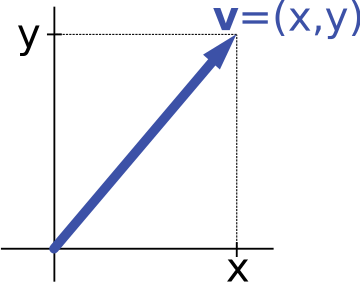
\includegraphics{images/Vector_components.png}
\caption{vectors}
\end{figure}

This is done to indicate that vectors have direction.

    \hypertarget{vector-arithmetic}{%
\paragraph{1.1.2 Vector arithmetic}\label{vector-arithmetic}}

Linear algebra \emph{is} algebra, and comes with generalizations of all
of our favorite arithmetic operations. In fact, when working with
columns and rows of data, we're actually doing vector arithmetic
operations. So, what are they and how are they done?

    \hypertarget{addition-and-subtraction}{%
\paragraph{1.1.2.1 Addition and
subtraction}\label{addition-and-subtraction}}

For vectors, addition and subtraction is ``pointwise'' and only works
with same-size (dimension) vectors. Pointwise addition between
\(u = [u_1,u_2, \cdots,u_n]\) and \(v = [v_1,v_2, \cdots,v_n]\) means
the following: \[u + v = [u_1+v_1, u_2+v_2, \cdots, u_n+v_n]\]
Graphically, here's what's going on when you add two vectors together:

\begin{figure}
\centering
\includegraphics{images/uv-addition.gif}
\caption{uv addition}
\end{figure}

We can do vector addition/subtraction by using numpy. Specifically, when
we run \texttt{np.array()} on a list the resulting object works like a
vector and handles the rest for us!

    \begin{Verbatim}[commandchars=\\\{\}]
{\color{incolor}In [{\color{incolor}36}]:} \PY{n}{u} \PY{o}{=} \PY{n}{np}\PY{o}{.}\PY{n}{array}\PY{p}{(}\PY{p}{[}\PY{o}{\PYZhy{}}\PY{l+m+mf}{5.}\PY{p}{,} \PY{l+m+mf}{3.7}\PY{p}{,} \PY{l+m+mf}{2.}\PY{p}{,} \PY{l+m+mf}{10.}\PY{p}{,} \PY{l+m+mf}{0.}\PY{p}{]}\PY{p}{)}
         \PY{n+nb}{print}\PY{p}{(}\PY{n}{u}\PY{p}{)}
         
         \PY{n}{v} \PY{o}{=} \PY{n}{np}\PY{o}{.}\PY{n}{array}\PY{p}{(}\PY{p}{[}\PY{l+m+mf}{9.}\PY{p}{,} \PY{l+m+mf}{2.}\PY{p}{,} \PY{l+m+mf}{4.}\PY{p}{,} \PY{l+m+mf}{8.}\PY{p}{,} \PY{l+m+mf}{1.}\PY{p}{]}\PY{p}{)}
         \PY{n+nb}{print}\PY{p}{(}\PY{n}{v}\PY{p}{)}
         \PY{n+nb}{print}\PY{p}{(}\PY{n}{u} \PY{o}{+} \PY{n}{v}\PY{p}{)}
\end{Verbatim}


    \begin{Verbatim}[commandchars=\\\{\}]
[-5.   3.7  2.  10.   0. ]
[9. 2. 4. 8. 1.]
[ 4.   5.7  6.  18.   1. ]

    \end{Verbatim}

    \hypertarget{exercise-vector-arithmetic}{%
\paragraph{1.1.2.2 Exercise: vector
arithmetic}\label{exercise-vector-arithmetic}}

Calculate \texttt{A} - \texttt{B} for the provided vectors, without
using a loop.

    \begin{Verbatim}[commandchars=\\\{\}]
{\color{incolor}In [{\color{incolor}37}]:} \PY{n}{A} \PY{o}{=} \PY{p}{[}\PY{n}{i} \PY{k}{for} \PY{n}{i} \PY{o+ow}{in} \PY{n+nb}{range}\PY{p}{(}\PY{l+m+mi}{5}\PY{p}{)}\PY{p}{]}
         \PY{n}{B} \PY{o}{=} \PY{p}{[}\PY{o}{\PYZhy{}}\PY{n}{i} \PY{k}{for} \PY{n}{i} \PY{o+ow}{in} \PY{n+nb}{range}\PY{p}{(}\PY{l+m+mi}{5}\PY{p}{)}\PY{p}{]}
         
         \PY{c+c1}{\PYZsh{} Answer goes here}
\end{Verbatim}


    \hypertarget{vector-norms}{%
\paragraph{1.1.2.3 Vector norms}\label{vector-norms}}

Some of the most important tools in the linear-algebra toolkit are
measures of bigness, or, norms. More precisely and for us in our study
of vectors, we can think of a \emph{norm} as a function that takes a
vector as input and outputs a non-negative quantity. Thus, a norm
\emph{measures} a vector, allowing us to define notions of distance,
which when ``normalized'' may allow us to, e.g., assess similarities and
other relationships between vectors.

For a vector \(v = [v_1,v_2, \cdots,v_n]\), its norm (size) is indicated
by \(\|v\|\), and in Euclidean, i.e., striaght-line-distance space, it's
computed as: \[\|v\| = \sqrt{v_1^2 + v_2^2 + \cdots + v_n^2}\]

According to the above, in base Python we'd have to square the
components of a vector (i.e., squared it pointwise), add them up, and
take the square-root to produce its Eucliudean norm. Now that we have a
computational framework to perform linerar algebra, norms (like
averages) can be processed abstractly with a built-in \texttt{numpy}
function: \texttt{numpy.linalg.norm()} (the default is the euclidean
norm). Note: this function also does other norms, like the taxicab norm,
which measures distances according to zig-zag pathways.

    \begin{Verbatim}[commandchars=\\\{\}]
{\color{incolor}In [{\color{incolor}38}]:} \PY{n}{v} \PY{o}{=} \PY{n}{np}\PY{o}{.}\PY{n}{array}\PY{p}{(}\PY{p}{[}\PY{l+m+mf}{9.}\PY{p}{,} \PY{l+m+mf}{2.}\PY{p}{,} \PY{l+m+mf}{4.}\PY{p}{,} \PY{l+m+mf}{8.}\PY{p}{,} \PY{l+m+mf}{1.}\PY{p}{]}\PY{p}{)}
         \PY{n+nb}{print}\PY{p}{(}\PY{n}{v}\PY{p}{)}
         \PY{n+nb}{print}\PY{p}{(}\PY{n}{np}\PY{o}{.}\PY{n}{linalg}\PY{o}{.}\PY{n}{norm}\PY{p}{(}\PY{n}{v}\PY{p}{)}\PY{p}{)}
\end{Verbatim}


    \begin{Verbatim}[commandchars=\\\{\}]
[9. 2. 4. 8. 1.]
12.884098726725126

    \end{Verbatim}

    \hypertarget{scalar-multiplication}{%
\paragraph{1.1.2.4 Scalar multiplication}\label{scalar-multiplication}}

Note: vector multiplication is less straightforward than addition and
comes in flavors. We'll go through these, building up in complexity.

Scalar multiplication just means multiplying a vector by a constant. So,
in this case every single value of a vector is multiplied the usual way
by the constant value. If we have a vector
\(v = [v_1, v_2, \cdots, v_n]\) and a constant, \(c\), their product is
\[cv = [cv_1, cv_2, \cdots, cv_n]\]

This is specifically called scalar multiplication because it scales,
i.e., grows/shrinks vectors by a constant amount in all directions:

\begin{figure}
\centering
\includegraphics{images/scaledvector.gif}
\caption{scaled vector}
\end{figure}

Scalar multiplication is also super easy when you have a number and a
numpy array:

    \begin{Verbatim}[commandchars=\\\{\}]
{\color{incolor}In [{\color{incolor}39}]:} \PY{n}{v} \PY{o}{=} \PY{n}{np}\PY{o}{.}\PY{n}{array}\PY{p}{(}\PY{p}{[}\PY{l+m+mf}{9.}\PY{p}{,} \PY{l+m+mf}{2.}\PY{p}{,} \PY{l+m+mf}{4.}\PY{p}{,} \PY{l+m+mf}{8.}\PY{p}{,} \PY{l+m+mf}{1.}\PY{p}{]}\PY{p}{)}
         \PY{n+nb}{print}\PY{p}{(}\PY{n}{v}\PY{p}{)}
         
         \PY{n}{c} \PY{o}{=} \PY{l+m+mf}{3.}
         \PY{n+nb}{print}\PY{p}{(}\PY{n}{c}\PY{p}{)}
         \PY{n+nb}{print}\PY{p}{(}\PY{n}{c} \PY{o}{*} \PY{n}{v}\PY{p}{)}
\end{Verbatim}


    \begin{Verbatim}[commandchars=\\\{\}]
[9. 2. 4. 8. 1.]
3.0
[27.  6. 12. 24.  3.]

    \end{Verbatim}

    \hypertarget{exercise-scalar-multiplication}{%
\paragraph{1.1.2.5 Exercise: scalar
multiplication}\label{exercise-scalar-multiplication}}

Divide each element in the above vector \texttt{v} by 4.

    \begin{Verbatim}[commandchars=\\\{\}]
{\color{incolor}In [{\color{incolor}40}]:} \PY{c+c1}{\PYZsh{} Answer goes here.}
\end{Verbatim}


    \hypertarget{pointwise-multiplication}{%
\paragraph{1.1.2.6 Pointwise
multiplication}\label{pointwise-multiplication}}

This is what numpy does with two vectors by default. Here, ``pointwise''
once again means that the first elements are multiplied together, second
elements are multiplied together, etc., to produce another vector of the
same length. So, pointwise multiplication between
\(u = [u_1,u_2, \cdots,u_n]\) and \(v = [v_1,v_2, \cdots,v_n]\) means
the following: \[uv = [u_1v_1, u_2v_2, \cdots, u_nv_n]\]

While pointwise products are super useful to us for data handling and
come up quite alot, they are not, on their own, particularly intuitively
visualizable, and for this mathematical branch, are most often used as a
step taken towards a different kind of product that we'll discuss next.
However, pointwise products are once again quite easy and useful with
numpy:

    \begin{Verbatim}[commandchars=\\\{\}]
{\color{incolor}In [{\color{incolor}41}]:} \PY{n}{u} \PY{o}{=} \PY{n}{np}\PY{o}{.}\PY{n}{array}\PY{p}{(}\PY{p}{[}\PY{o}{\PYZhy{}}\PY{l+m+mf}{5.}\PY{p}{,} \PY{l+m+mf}{3.7}\PY{p}{,} \PY{l+m+mf}{2.}\PY{p}{,} \PY{l+m+mf}{10.}\PY{p}{,} \PY{l+m+mf}{0.}\PY{p}{]}\PY{p}{)}
         \PY{n+nb}{print}\PY{p}{(}\PY{n}{u}\PY{p}{)}
         
         \PY{n}{v} \PY{o}{=} \PY{n}{np}\PY{o}{.}\PY{n}{array}\PY{p}{(}\PY{p}{[}\PY{l+m+mf}{9.}\PY{p}{,} \PY{l+m+mf}{2.}\PY{p}{,} \PY{l+m+mf}{4.}\PY{p}{,} \PY{l+m+mf}{8.}\PY{p}{,} \PY{l+m+mf}{1.}\PY{p}{]}\PY{p}{)}
         \PY{n+nb}{print}\PY{p}{(}\PY{n}{v}\PY{p}{)}
         \PY{n+nb}{print}\PY{p}{(}\PY{n}{u} \PY{o}{*} \PY{n}{v}\PY{p}{)}
\end{Verbatim}


    \begin{Verbatim}[commandchars=\\\{\}]
[-5.   3.7  2.  10.   0. ]
[9. 2. 4. 8. 1.]
[-45.    7.4   8.   80.    0. ]

    \end{Verbatim}

    \hypertarget{exercise-pointwise-vector-multiplication}{%
\paragraph{1.1.2.7 Exercise: pointwise vector
multiplication}\label{exercise-pointwise-vector-multiplication}}

Perform pointwise multiplication between \texttt{v} divided by 4 which
you calculated above, and \texttt{u}.

    \begin{Verbatim}[commandchars=\\\{\}]
{\color{incolor}In [{\color{incolor}42}]:} \PY{c+c1}{\PYZsh{} Answer goes here.}
\end{Verbatim}


    \hypertarget{inner-products}{%
\paragraph{1.1.2.8 Inner products}\label{inner-products}}

This is just the sum of a pointwise product. While inner (a.k.a ``dot'')
products build off of the pointwise product, they tell us about a lot
more. Specifically, when two non-zero vectors have an inner product of
\(0\), they are orthogonal. Orthogonality is the fancy-math word for
perpindicular when you're dealing with more than two dimensions. So, an
inner product between \(u = [u_1,u_2, \cdots,u_n]\) and
\(v = [v_1,v_2, \cdots,v_n]\) results in the scalar value---not a
vector---produced by the following fomula:
\[u\cdot v = u_1v_1+u_2v_2+\cdots+u_nv_n\]

Intuitively, an inner product helps describe the projected length of one
vector onto another. In particular, naming \(u_v\) and \(v_u\) as the
projections of \(v\) onto \(u\) and \(u\) onto \(v\), respectively, we
have: \[u\cdot v = u_v\|v\| = v_u\|u\|\]

So, when two vectors are a right-angle off of one another, their
projections have length zero. Here's a graphical depiction of this
intuitive description of an inner product:

\begin{figure}
\centering
\includegraphics{images/projection.gif}
\caption{inner}
\end{figure}

Now, if we want to find the inner product between two vectors, all we
have to do is add up their pointwise product:

    \begin{Verbatim}[commandchars=\\\{\}]
{\color{incolor}In [{\color{incolor}43}]:} \PY{n}{u} \PY{o}{=} \PY{n}{np}\PY{o}{.}\PY{n}{array}\PY{p}{(}\PY{p}{[}\PY{o}{\PYZhy{}}\PY{l+m+mf}{5.}\PY{p}{,} \PY{l+m+mf}{3.7}\PY{p}{,} \PY{l+m+mf}{2.}\PY{p}{,} \PY{l+m+mf}{10.}\PY{p}{,} \PY{l+m+mf}{0.}\PY{p}{]}\PY{p}{)}
         \PY{n+nb}{print}\PY{p}{(}\PY{n}{u}\PY{p}{)}
         
         \PY{n}{v} \PY{o}{=} \PY{n}{np}\PY{o}{.}\PY{n}{array}\PY{p}{(}\PY{p}{[}\PY{l+m+mf}{9.}\PY{p}{,} \PY{l+m+mf}{2.}\PY{p}{,} \PY{l+m+mf}{4.}\PY{p}{,} \PY{l+m+mf}{8.}\PY{p}{,} \PY{l+m+mf}{1.}\PY{p}{]}\PY{p}{)}
         \PY{n+nb}{print}\PY{p}{(}\PY{n}{v}\PY{p}{)}
         \PY{n+nb}{print}\PY{p}{(}\PY{n+nb}{sum}\PY{p}{(}\PY{n}{u} \PY{o}{*} \PY{n}{v}\PY{p}{)}\PY{p}{)}
\end{Verbatim}


    \begin{Verbatim}[commandchars=\\\{\}]
[-5.   3.7  2.  10.   0. ]
[9. 2. 4. 8. 1.]
50.4

    \end{Verbatim}

    However, the numpy way to do this uses the \texttt{.dot()} method on an
array. Recall: the inner product is also called the dot product.

    \begin{Verbatim}[commandchars=\\\{\}]
{\color{incolor}In [{\color{incolor}44}]:} \PY{n}{u} \PY{o}{=} \PY{n}{np}\PY{o}{.}\PY{n}{array}\PY{p}{(}\PY{p}{[}\PY{o}{\PYZhy{}}\PY{l+m+mf}{5.}\PY{p}{,} \PY{l+m+mf}{3.7}\PY{p}{,} \PY{l+m+mf}{2.}\PY{p}{,} \PY{l+m+mf}{10.}\PY{p}{,} \PY{l+m+mf}{0.}\PY{p}{]}\PY{p}{)}
         \PY{n+nb}{print}\PY{p}{(}\PY{n}{u}\PY{p}{)}
         
         \PY{n}{v} \PY{o}{=} \PY{n}{np}\PY{o}{.}\PY{n}{array}\PY{p}{(}\PY{p}{[}\PY{l+m+mf}{9.}\PY{p}{,} \PY{l+m+mf}{2.}\PY{p}{,} \PY{l+m+mf}{4.}\PY{p}{,} \PY{l+m+mf}{8.}\PY{p}{,} \PY{l+m+mf}{1.}\PY{p}{]}\PY{p}{)}
         \PY{n+nb}{print}\PY{p}{(}\PY{n}{v}\PY{p}{)}
         \PY{n+nb}{print}\PY{p}{(}\PY{n}{u}\PY{o}{.}\PY{n}{dot}\PY{p}{(}\PY{n}{v}\PY{p}{)}\PY{p}{)}
\end{Verbatim}


    \begin{Verbatim}[commandchars=\\\{\}]
[-5.   3.7  2.  10.   0. ]
[9. 2. 4. 8. 1.]
50.4

    \end{Verbatim}

    \hypertarget{exercise-inner-products}{%
\paragraph{1.1.2.9 Exercise: inner
products}\label{exercise-inner-products}}

Find the dot product of the provided array \texttt{z} with the dot
product of \texttt{u} and \texttt{v}, from above.

    \begin{Verbatim}[commandchars=\\\{\}]
{\color{incolor}In [{\color{incolor}45}]:} \PY{n}{z} \PY{o}{=} \PY{n}{np}\PY{o}{.}\PY{n}{array}\PY{p}{(}\PY{p}{[}\PY{l+m+mi}{1}\PY{p}{,} \PY{l+m+mi}{2}\PY{p}{,} \PY{l+m+mi}{3}\PY{p}{,} \PY{l+m+mi}{4}\PY{p}{,} \PY{l+m+mi}{5}\PY{p}{]}\PY{p}{)}
         
         \PY{c+c1}{\PYZsh{} Answer goes here.}
\end{Verbatim}


    \hypertarget{example-defining-similarity-hence-correlation-with-vector-products}{%
\paragraph{1.1.2.10 Example: defining similarity (hence correlation)
with vector
products}\label{example-defining-similarity-hence-correlation-with-vector-products}}

Inner product makes it really easy to define distance and similarity,
and thus for the statistical world, correlation.

In our exploraton of descriptive statistics and exploratory data
analysis (\textbf{Chapter 3}) we'll spend significant time building up
from distance measures to arrive at a balanced data-comparison method
called the correlation. Along the way, an important stop is a similarity
measure called \emph{cosine similarity}. This takes effort to express in
terms of concepts like means and variances, but with our linear algebra
formalism at our disposal can express similarity succinctly:
\[sim(u,v) = \frac{u\cdot v}{\|u\|\|v\|}\]

Moreover, we can compute it quickly using the fancy numpy method
\texttt{.dot()} (below), and intuit that the relationships entailed by
correlation actually have to do with projection (note the dot/inner
product above), i.e., the extent to which one vector (of numerical data)
points along the direction of another. As we'll discuss in
\textbf{Chapter 3}, the cosine (it can also be computed
trigonometrically) similarity is a number derived from a pair of vectors
that ranges over \texttt{{[}-1,1{]}}, which indicates how related they
are: a value close to \(0\) indicates little or no relationship exists,
while values close to \(1\) or \(-1\) indicate when vectors positively
(point along the same directions) or negatively (point along opposing
directions) associate, respectively.

    \begin{Verbatim}[commandchars=\\\{\}]
{\color{incolor}In [{\color{incolor}46}]:} \PY{n}{u} \PY{o}{=} \PY{n}{np}\PY{o}{.}\PY{n}{array}\PY{p}{(}\PY{p}{[}\PY{o}{\PYZhy{}}\PY{l+m+mf}{5.}\PY{p}{,} \PY{l+m+mf}{3.7}\PY{p}{,} \PY{l+m+mf}{2.}\PY{p}{,} \PY{l+m+mf}{10.}\PY{p}{,} \PY{l+m+mf}{0.}\PY{p}{]}\PY{p}{)}
         \PY{n+nb}{print}\PY{p}{(}\PY{n}{u}\PY{p}{)}
         
         \PY{n}{v} \PY{o}{=} \PY{n}{np}\PY{o}{.}\PY{n}{array}\PY{p}{(}\PY{p}{[}\PY{l+m+mf}{9.}\PY{p}{,} \PY{l+m+mf}{2.}\PY{p}{,} \PY{l+m+mf}{4.}\PY{p}{,} \PY{l+m+mf}{8.}\PY{p}{,} \PY{l+m+mf}{1.}\PY{p}{]}\PY{p}{)}
         \PY{n+nb}{print}\PY{p}{(}\PY{n}{v}\PY{p}{)}
         
         \PY{n}{sim} \PY{o}{=} \PY{n}{u}\PY{o}{.}\PY{n}{dot}\PY{p}{(}\PY{n}{v}\PY{p}{)} \PY{o}{/} \PY{p}{(}\PY{n}{np}\PY{o}{.}\PY{n}{linalg}\PY{o}{.}\PY{n}{norm}\PY{p}{(}\PY{n}{u}\PY{p}{)} \PY{o}{*} \PY{n}{np}\PY{o}{.}\PY{n}{linalg}\PY{o}{.}\PY{n}{norm}\PY{p}{(}\PY{n}{v}\PY{p}{)}\PY{p}{)}
         \PY{n+nb}{print}\PY{p}{(}\PY{n}{sim}\PY{p}{)}
\end{Verbatim}


    \begin{Verbatim}[commandchars=\\\{\}]
[-5.   3.7  2.  10.   0. ]
[9. 2. 4. 8. 1.]
0.32747618583046045

    \end{Verbatim}

    \hypertarget{exercise-cosine-similarity}{%
\paragraph{1.1.2.11 Exercise: cosine
similarity}\label{exercise-cosine-similarity}}

Find the cosine similarity of the vectors \texttt{a} and \texttt{b}.

    \begin{Verbatim}[commandchars=\\\{\}]
{\color{incolor}In [{\color{incolor}47}]:} \PY{n}{a} \PY{o}{=} \PY{n}{np}\PY{o}{.}\PY{n}{array}\PY{p}{(}\PY{p}{[}\PY{l+m+mi}{1}\PY{p}{,} \PY{l+m+mi}{0}\PY{p}{,} \PY{l+m+mi}{0}\PY{p}{]}\PY{p}{)}
         \PY{n}{b} \PY{o}{=} \PY{n}{np}\PY{o}{.}\PY{n}{array}\PY{p}{(}\PY{p}{[}\PY{l+m+mi}{0}\PY{p}{,} \PY{l+m+mi}{1}\PY{p}{,} \PY{l+m+mi}{0}\PY{p}{]}\PY{p}{)}
         
         \PY{c+c1}{\PYZsh{} Answer goes here}
\end{Verbatim}


    \hypertarget{matrices}{%
\subsubsection{1.1.3 Matrices}\label{matrices}}

If it helps to think about vectors as the rows and columns of a
spreadsheet, then think of the whole spreadsheet as a matrix---a
collection of vectors (i.e., rows or columns) of the same length. More
generally, a matrix is a two-dimensional ordered-array of numbers:

\[ A = \begin{bmatrix} a_{1,1} & a_{1,2} & \dots & a_{1,n} \\ a_{2,1} & a_{2,2} & \dots & a_{2,n} \\ \vdots & \vdots & \ddots & \vdots \\ a_{m,1} & a_{m,2} & \dots & a_{m,n} \end{bmatrix} \]

While we could take a list of equal-length lists of numbers as a basic
way to represet matrices in Python, numpy has already built in some very
nice object types for working with matrices and performing matrix
operations. Since there are now two dimensions of data inside of a a
matrix it helps to get a bit of notation straight: when describing the
numbers of rows and columns in a matrix it is conventional to list these
numbers as row-by-column. So, an \(m \times n\) matrix, \(A\), has \(m\)
rows and \(n\) columns. Likewise, when indexing to indicate the
individual elements of an \(A\) it is customary to indicate the row
position first, followed by the column position. So, the element
\(a_{i,j}\) refers to the number in the \(i^\text{th}\) row and
\(j^\text{th}\) column of \(A\).

\hypertarget{casting-matrices-with-numpy.array}{%
\paragraph{\texorpdfstring{1.1.3.1 Casting matrices with
\texttt{numpy.array()}}{1.1.3.1 Casting matrices with numpy.array()}}\label{casting-matrices-with-numpy.array}}

We can define matrices easily in numpy by using \texttt{numpy.array()}
on lists of same-length lists:

    \begin{Verbatim}[commandchars=\\\{\}]
{\color{incolor}In [{\color{incolor}62}]:} \PY{c+c1}{\PYZsh{}\PYZsh{} define a 4\PYZhy{}row by 3\PYZhy{}column matrix}
         \PY{n}{A} \PY{o}{=} \PY{n}{np}\PY{o}{.}\PY{n}{array}\PY{p}{(}\PY{p}{[}
             \PY{p}{[}\PY{l+m+mi}{1}\PY{p}{,} \PY{l+m+mi}{2}\PY{p}{,} \PY{l+m+mi}{3}\PY{p}{]}\PY{p}{,}
             \PY{p}{[}\PY{l+m+mi}{4}\PY{p}{,} \PY{l+m+mi}{5}\PY{p}{,} \PY{l+m+mi}{6}\PY{p}{]}\PY{p}{,}
             \PY{p}{[}\PY{l+m+mi}{7}\PY{p}{,} \PY{l+m+mi}{8}\PY{p}{,} \PY{l+m+mi}{9}\PY{p}{]}\PY{p}{,}
             \PY{p}{[}\PY{l+m+mi}{10}\PY{p}{,} \PY{l+m+mi}{11}\PY{p}{,} \PY{l+m+mi}{12}\PY{p}{]}
         \PY{p}{]}\PY{p}{)}
         
         \PY{n+nb}{print}\PY{p}{(}\PY{n}{A}\PY{p}{)}
\end{Verbatim}


    \begin{Verbatim}[commandchars=\\\{\}]
[[ 1  2  3]
 [ 4  5  6]
 [ 7  8  9]
 [10 11 12]]

    \end{Verbatim}

    \hypertarget{d-matrix-indexing}{%
\paragraph{1.1.3.2 (2-d) Matrix indexing}\label{d-matrix-indexing}}

Numpy still uses python 0-indexing, but matrices take two indices to
access individual elements. In line with the discussion in
\textbf{Section 1.1.2}, this is row-by-column:

    \begin{Verbatim}[commandchars=\\\{\}]
{\color{incolor}In [{\color{incolor}67}]:} \PY{c+c1}{\PYZsh{}\PYZsh{} define a 4\PYZhy{}row by 3\PYZhy{}column matrix}
         \PY{n}{A} \PY{o}{=} \PY{n}{np}\PY{o}{.}\PY{n}{array}\PY{p}{(}\PY{p}{[}
             \PY{p}{[} \PY{l+m+mi}{1}\PY{p}{,}  \PY{l+m+mi}{2}\PY{p}{,}  \PY{l+m+mi}{3}\PY{p}{]}\PY{p}{,}
             \PY{p}{[} \PY{l+m+mi}{4}\PY{p}{,}  \PY{l+m+mi}{5}\PY{p}{,}  \PY{l+m+mi}{6}\PY{p}{]}\PY{p}{,}
             \PY{p}{[} \PY{l+m+mi}{7}\PY{p}{,}  \PY{l+m+mi}{8}\PY{p}{,}  \PY{l+m+mi}{9}\PY{p}{]}\PY{p}{,}
             \PY{p}{[}\PY{l+m+mi}{10}\PY{p}{,} \PY{l+m+mi}{11}\PY{p}{,} \PY{l+m+mi}{12}\PY{p}{]}
         \PY{p}{]}\PY{p}{)}
         
         \PY{n+nb}{print}\PY{p}{(}\PY{n}{A}\PY{p}{)}
         
         \PY{c+c1}{\PYZsh{}\PYZsh{} pull out the value in row 2, column 3}
         \PY{n+nb}{print}\PY{p}{(}\PY{n}{A}\PY{p}{[}\PY{l+m+mi}{1}\PY{p}{,} \PY{l+m+mi}{2}\PY{p}{]}\PY{p}{)}
\end{Verbatim}


    \begin{Verbatim}[commandchars=\\\{\}]
[[ 1  2  3]
 [ 4  5  6]
 [ 7  8  9]
 [10 11 12]]
6

    \end{Verbatim}

    \hypertarget{exercise-matrix-indexing}{%
\paragraph{1.1.3.3 Exercise: Matrix
indexing}\label{exercise-matrix-indexing}}

Print the value in the above matrix \texttt{A} located in the
bottom-right entry.

    \begin{Verbatim}[commandchars=\\\{\}]
{\color{incolor}In [{\color{incolor}50}]:} \PY{c+c1}{\PYZsh{} Answer goes here.}
\end{Verbatim}


    \hypertarget{transposition}{%
\paragraph{1.1.3.4 Transposition}\label{transposition}}

In line with matrices' (2-d \texttt{array}'s) alignment to their
mathematical construct, they have built-in function for
\emph{transposition}, which switches rows and columns:

\[ A^T = \begin{bmatrix} a_{1,1} & a_{2,1} & \dots & a_{m,1} \\ a_{1,2} & a_{2,2} & \dots & a_{m,2} \\ \vdots & \vdots & \ddots & \vdots \\ a_{1,n} & a_{2,n} & \dots & a_{m,n} \end{bmatrix} \]

So, not only can one take the above (cast with \texttt{np.array()}) and
transpose it by running \texttt{A.transpose()}, but it can otherwise be
performed easily by the module on external objects (like lists of
lists), using \texttt{np.transpose()}:

    \begin{Verbatim}[commandchars=\\\{\}]
{\color{incolor}In [{\color{incolor}51}]:} \PY{c+c1}{\PYZsh{}\PYZsh{} define a 4\PYZhy{}row by 3\PYZhy{}column matrix}
         \PY{n}{A} \PY{o}{=} \PY{n}{np}\PY{o}{.}\PY{n}{array}\PY{p}{(}\PY{p}{[}
             \PY{p}{[}\PY{l+m+mi}{1}\PY{p}{,} \PY{l+m+mi}{2}\PY{p}{,} \PY{l+m+mi}{3}\PY{p}{]}\PY{p}{,}
             \PY{p}{[}\PY{l+m+mi}{4}\PY{p}{,} \PY{l+m+mi}{5}\PY{p}{,} \PY{l+m+mi}{6}\PY{p}{]}\PY{p}{,}
             \PY{p}{[}\PY{l+m+mi}{7}\PY{p}{,} \PY{l+m+mi}{8}\PY{p}{,} \PY{l+m+mi}{9}\PY{p}{]}\PY{p}{,}
             \PY{p}{[}\PY{l+m+mi}{10}\PY{p}{,} \PY{l+m+mi}{11}\PY{p}{,} \PY{l+m+mi}{12}\PY{p}{]}
         \PY{p}{]}\PY{p}{)}
         
         \PY{c+c1}{\PYZsh{}\PYZsh{} take the matrix transpose}
         \PY{n+nb}{print}\PY{p}{(}\PY{n}{np}\PY{o}{.}\PY{n}{transpose}\PY{p}{(}\PY{n}{A}\PY{p}{)}\PY{p}{)}
         \PY{n+nb}{print}\PY{p}{(}\PY{p}{)}
         \PY{n+nb}{print}\PY{p}{(}\PY{n}{A}\PY{o}{.}\PY{n}{transpose}\PY{p}{(}\PY{p}{)}\PY{p}{)}
\end{Verbatim}


    \begin{Verbatim}[commandchars=\\\{\}]
[[ 1  4  7 10]
 [ 2  5  8 11]
 [ 3  6  9 12]]

[[ 1  4  7 10]
 [ 2  5  8 11]
 [ 3  6  9 12]]

    \end{Verbatim}

    \hypertarget{matrix-arithmetic}{%
\subsubsection{1.1.4 Matrix arithmetic}\label{matrix-arithmetic}}

Like vectors, matrices have their own arithmetic and it is largely an
extension or generalization of what is done for vectors. Numpy likewise
has lots of good built-in functionality for this.

\hypertarget{addition-subtraction}{%
\paragraph{1.1.4.1 Addition \& Subtraction}\label{addition-subtraction}}

For two same-dimension matrices, addition is once again pointwise, but
now according to row-column, i.e., \(i,j\)-position:

\[ A + B = \begin{bmatrix} a_{1,1} + b_{1,1} & a_{1,2} + b_{1,2} & \dots & a_{1,n} + b_{1,n} \\ a_{2,1} + b_{2,1} & a_{2,2} + b_{2,2} & \dots & a_{2,n} + b_{2,n} \\ \vdots & \vdots & \ddots & \vdots \\ a_{m,1} + b_{m,1} & a_{m,2} + b_{m,2} & \dots & a_{m,n} + b_{m,n} \end{bmatrix} \]

As it turns out, this is precisely what numpy does by default when you
add two arrays:

    \begin{Verbatim}[commandchars=\\\{\}]
{\color{incolor}In [{\color{incolor}52}]:} \PY{c+c1}{\PYZsh{}\PYZsh{} define a 4\PYZhy{}row by 3\PYZhy{}column matrix}
         \PY{n}{A} \PY{o}{=} \PY{n}{np}\PY{o}{.}\PY{n}{array}\PY{p}{(}\PY{p}{[}
             \PY{p}{[} \PY{l+m+mi}{1}\PY{p}{,}  \PY{l+m+mi}{2}\PY{p}{,}  \PY{l+m+mi}{3}\PY{p}{]}\PY{p}{,}
             \PY{p}{[} \PY{l+m+mi}{4}\PY{p}{,}  \PY{l+m+mi}{5}\PY{p}{,}  \PY{l+m+mi}{6}\PY{p}{]}\PY{p}{,}
             \PY{p}{[} \PY{l+m+mi}{7}\PY{p}{,}  \PY{l+m+mi}{8}\PY{p}{,}  \PY{l+m+mi}{9}\PY{p}{]}\PY{p}{,}
             \PY{p}{[}\PY{l+m+mi}{10}\PY{p}{,} \PY{l+m+mi}{11}\PY{p}{,} \PY{l+m+mi}{12}\PY{p}{]}
         \PY{p}{]}\PY{p}{)}
         
         \PY{n+nb}{print}\PY{p}{(}\PY{n}{A}\PY{p}{,} \PY{l+s+s1}{\PYZsq{}}\PY{l+s+se}{\PYZbs{}n}\PY{l+s+s1}{\PYZsq{}}\PY{p}{)}
         
         \PY{c+c1}{\PYZsh{}\PYZsh{} define another 4\PYZhy{}row by 3\PYZhy{}column matrix}
         \PY{n}{B} \PY{o}{=} \PY{n}{np}\PY{o}{.}\PY{n}{array}\PY{p}{(}\PY{p}{[}
             \PY{p}{[} \PY{l+m+mi}{11}\PY{p}{,}  \PY{l+m+mi}{12}\PY{p}{,}  \PY{l+m+mi}{13}\PY{p}{]}\PY{p}{,}
             \PY{p}{[} \PY{l+m+mi}{14}\PY{p}{,}  \PY{l+m+mi}{15}\PY{p}{,}  \PY{l+m+mi}{16}\PY{p}{]}\PY{p}{,}
             \PY{p}{[} \PY{l+m+mi}{17}\PY{p}{,}  \PY{l+m+mi}{18}\PY{p}{,}  \PY{l+m+mi}{19}\PY{p}{]}\PY{p}{,}
             \PY{p}{[} \PY{l+m+mi}{20}\PY{p}{,}  \PY{l+m+mi}{21}\PY{p}{,}  \PY{l+m+mi}{22}\PY{p}{]}
         \PY{p}{]}\PY{p}{)}
         
         \PY{n+nb}{print}\PY{p}{(}\PY{n}{B}\PY{p}{,} \PY{l+s+s1}{\PYZsq{}}\PY{l+s+se}{\PYZbs{}n}\PY{l+s+s1}{\PYZsq{}}\PY{p}{)}
         
         \PY{c+c1}{\PYZsh{}\PYZsh{} take the matrix sum of the two}
         \PY{n+nb}{print}\PY{p}{(}\PY{n}{A} \PY{o}{+} \PY{n}{B}\PY{p}{)}
\end{Verbatim}


    \begin{Verbatim}[commandchars=\\\{\}]
[[ 1  2  3]
 [ 4  5  6]
 [ 7  8  9]
 [10 11 12]] 

[[11 12 13]
 [14 15 16]
 [17 18 19]
 [20 21 22]] 

[[12 14 16]
 [18 20 22]
 [24 26 28]
 [30 32 34]]

    \end{Verbatim}

    \hypertarget{exercise-matrix-addition}{%
\paragraph{1.1.4.2 Exercise: matrix
addition}\label{exercise-matrix-addition}}

Using \texttt{A} and \texttt{B} from above, find the sum \texttt{A} +
\texttt{B} + \texttt{A}.

    \begin{Verbatim}[commandchars=\\\{\}]
{\color{incolor}In [{\color{incolor}53}]:} \PY{c+c1}{\PYZsh{} Answer goes here.}
\end{Verbatim}


    \hypertarget{scalar-matrix-multiplication}{%
\paragraph{1.1.4.3 Scalar matrix
multiplication}\label{scalar-matrix-multiplication}}

As with vectors, multiplication comes in multiple different flavors, and
just like matrices make things more complicated, their multiplication is
more complicated, too. However, like with vectors we'll start with the
simplest forms possible and build up to what we need.

Multiplication by a scalar just multiplies every element. So, if we take
an \(m \times n\) matrix \(A\) and multiple it by a scalar (constant),
\(c\), we just get a \(c\)-grown or -shrunk version of the same:
\[ cA = \begin{bmatrix} ca_{1,1} & ca_{1,2} & \dots & ca_{1,n} \\ ca_{2,1} & ca_{2,2} & \dots & ca_{2,n} \\ \vdots & \vdots & \ddots & \vdots \\ ca_{m,1} & ca_{m,2} & \dots & ca_{m,n} \end{bmatrix} \]

This is likewise what numpy does with scalars and matrices by default:

    \begin{Verbatim}[commandchars=\\\{\}]
{\color{incolor}In [{\color{incolor}54}]:} \PY{c+c1}{\PYZsh{}\PYZsh{} define a 4\PYZhy{}row by 3\PYZhy{}column matrix}
         \PY{n}{A} \PY{o}{=} \PY{n}{np}\PY{o}{.}\PY{n}{array}\PY{p}{(}\PY{p}{[}
             \PY{p}{[} \PY{l+m+mi}{1}\PY{p}{,}  \PY{l+m+mi}{2}\PY{p}{,}  \PY{l+m+mi}{3}\PY{p}{]}\PY{p}{,}
             \PY{p}{[} \PY{l+m+mi}{4}\PY{p}{,}  \PY{l+m+mi}{5}\PY{p}{,}  \PY{l+m+mi}{6}\PY{p}{]}\PY{p}{,}
             \PY{p}{[} \PY{l+m+mi}{7}\PY{p}{,}  \PY{l+m+mi}{8}\PY{p}{,}  \PY{l+m+mi}{9}\PY{p}{]}\PY{p}{,}
             \PY{p}{[}\PY{l+m+mi}{10}\PY{p}{,} \PY{l+m+mi}{11}\PY{p}{,} \PY{l+m+mi}{12}\PY{p}{]}
         \PY{p}{]}\PY{p}{)}
         
         \PY{n+nb}{print}\PY{p}{(}\PY{n}{A}\PY{p}{,} \PY{l+s+s1}{\PYZsq{}}\PY{l+s+se}{\PYZbs{}n}\PY{l+s+s1}{\PYZsq{}}\PY{p}{)}
         
         \PY{c+c1}{\PYZsh{}\PYZsh{} define a constant}
         \PY{n}{c} \PY{o}{=} \PY{l+m+mi}{10}
         
         \PY{c+c1}{\PYZsh{}\PYZsh{} take the matrix sum of the two}
         \PY{n+nb}{print}\PY{p}{(}\PY{n}{c} \PY{o}{*} \PY{n}{A}\PY{p}{)}
\end{Verbatim}


    \begin{Verbatim}[commandchars=\\\{\}]
[[ 1  2  3]
 [ 4  5  6]
 [ 7  8  9]
 [10 11 12]] 

[[ 10  20  30]
 [ 40  50  60]
 [ 70  80  90]
 [100 110 120]]

    \end{Verbatim}

    \hypertarget{exercise-scalar-matrix-multiplication}{%
\paragraph{1.1.4.4 Exercise: Scalar matrix
multiplication}\label{exercise-scalar-matrix-multiplication}}

Divide each element in the above matrix \texttt{A} by 4.

    \begin{Verbatim}[commandchars=\\\{\}]
{\color{incolor}In [{\color{incolor}55}]:} \PY{c+c1}{\PYZsh{} Answer goes here.}
\end{Verbatim}


    \hypertarget{pointwise-multiplication}{%
\paragraph{1.1.4.5 Pointwise
multiplication}\label{pointwise-multiplication}}

This requires same-dimension matrices. But just like other pointwise
operations, this kind of multiplication is straightforward and can be
performed just with the usual \texttt{*}, i.e., times operator in
Python:

    \begin{Verbatim}[commandchars=\\\{\}]
{\color{incolor}In [{\color{incolor}56}]:} \PY{c+c1}{\PYZsh{}\PYZsh{} define a 4\PYZhy{}row by 3\PYZhy{}column matrix}
         \PY{n}{A} \PY{o}{=} \PY{n}{np}\PY{o}{.}\PY{n}{array}\PY{p}{(}\PY{p}{[}
             \PY{p}{[} \PY{l+m+mi}{1}\PY{p}{,}  \PY{l+m+mi}{2}\PY{p}{,}  \PY{l+m+mi}{3}\PY{p}{]}\PY{p}{,}
             \PY{p}{[} \PY{l+m+mi}{4}\PY{p}{,}  \PY{l+m+mi}{5}\PY{p}{,}  \PY{l+m+mi}{6}\PY{p}{]}\PY{p}{,}
             \PY{p}{[} \PY{l+m+mi}{7}\PY{p}{,}  \PY{l+m+mi}{8}\PY{p}{,}  \PY{l+m+mi}{9}\PY{p}{]}\PY{p}{,}
             \PY{p}{[}\PY{l+m+mi}{10}\PY{p}{,} \PY{l+m+mi}{11}\PY{p}{,} \PY{l+m+mi}{12}\PY{p}{]}
         \PY{p}{]}\PY{p}{)}
         
         \PY{n+nb}{print}\PY{p}{(}\PY{n}{A}\PY{p}{,} \PY{l+s+s1}{\PYZsq{}}\PY{l+s+se}{\PYZbs{}n}\PY{l+s+s1}{\PYZsq{}}\PY{p}{)}
         
         \PY{c+c1}{\PYZsh{}\PYZsh{} define another 4\PYZhy{}row by 3\PYZhy{}column matrix}
         \PY{n}{B} \PY{o}{=} \PY{n}{np}\PY{o}{.}\PY{n}{array}\PY{p}{(}\PY{p}{[}
             \PY{p}{[} \PY{l+m+mi}{11}\PY{p}{,}  \PY{l+m+mi}{12}\PY{p}{,}  \PY{l+m+mi}{13}\PY{p}{]}\PY{p}{,}
             \PY{p}{[} \PY{l+m+mi}{14}\PY{p}{,}  \PY{l+m+mi}{15}\PY{p}{,}  \PY{l+m+mi}{16}\PY{p}{]}\PY{p}{,}
             \PY{p}{[} \PY{l+m+mi}{17}\PY{p}{,}  \PY{l+m+mi}{18}\PY{p}{,}  \PY{l+m+mi}{19}\PY{p}{]}\PY{p}{,}
             \PY{p}{[} \PY{l+m+mi}{20}\PY{p}{,}  \PY{l+m+mi}{21}\PY{p}{,}  \PY{l+m+mi}{22}\PY{p}{]}
         \PY{p}{]}\PY{p}{)}
         
         \PY{n+nb}{print}\PY{p}{(}\PY{n}{B}\PY{p}{,} \PY{l+s+s1}{\PYZsq{}}\PY{l+s+se}{\PYZbs{}n}\PY{l+s+s1}{\PYZsq{}}\PY{p}{)}
         
         \PY{c+c1}{\PYZsh{}\PYZsh{} take the pointwise matrix product of the two}
         \PY{n+nb}{print}\PY{p}{(}\PY{n}{A} \PY{o}{*} \PY{n}{B}\PY{p}{)}
\end{Verbatim}


    \begin{Verbatim}[commandchars=\\\{\}]
[[ 1  2  3]
 [ 4  5  6]
 [ 7  8  9]
 [10 11 12]] 

[[11 12 13]
 [14 15 16]
 [17 18 19]
 [20 21 22]] 

[[ 11  24  39]
 [ 56  75  96]
 [119 144 171]
 [200 231 264]]

    \end{Verbatim}

    \hypertarget{inner-products-of-matrices-and-vectors}{%
\paragraph{1.1.4.6 Inner products of matrices and
vectors}\label{inner-products-of-matrices-and-vectors}}

Here's the deal: a matrix times a vector equals another vector. But to
multiply a matrix by a vector there is one major stipulation: if \(A\)
is an \(m \times n\) matrix then you can only multiply \(A\) times a
vector, \(v\), as \(A\cdot v\) if \(v\) is an \(n \times 1\) column
vector. The result is then an \(m \times 1\) vector, which is once again
called the \emph{inner product}. Why? Because this is a
\emph{generalization of the inner product for vectors}. It works as
follows:

\[ \begin{align} A\cdot v & = \begin{bmatrix} a_{1,1} & a_{1,2} & \dots & a_{1,n} \\ a_{2,1} & a_{2,2} & \dots & a_{2,n} \\ \vdots & \vdots & \ddots & \vdots \\ a_{m,1} & a_{m,2} & \dots & a_{m,n} \end{bmatrix} \cdot \begin{bmatrix} v_{1} \\ v_{2} \\ \vdots \\ v_{n} \end{bmatrix}\\\\ & = \begin{bmatrix} a_{1,1}v_{1} + a_{1,2}v_{2} + \cdots + a_{1,n}v_{n} \\ a_{2,1}v_{1} + a_{2,2}v_{2} + \cdots + a_{2,n}v_{n} \\ \vdots \\ a_{m,1}v_{1} + a_{m,2}v_{2} + \cdots + a_{m,n}v_{n} \end{bmatrix} \end{align} \]

Taking the inner product of a matrix and a vector like this is once
again as straight forward as using the \texttt{.dot()} array method,
specifically in the order: \texttt{A.dot(v)}

    \begin{Verbatim}[commandchars=\\\{\}]
{\color{incolor}In [{\color{incolor}57}]:} \PY{c+c1}{\PYZsh{}\PYZsh{} define a 4\PYZhy{}row by 3\PYZhy{}column matrix}
         \PY{n}{A} \PY{o}{=} \PY{n}{np}\PY{o}{.}\PY{n}{array}\PY{p}{(}\PY{p}{[}
             \PY{p}{[} \PY{l+m+mi}{1}\PY{p}{,}  \PY{l+m+mi}{2}\PY{p}{,}  \PY{l+m+mi}{3}\PY{p}{]}\PY{p}{,}
             \PY{p}{[} \PY{l+m+mi}{4}\PY{p}{,}  \PY{l+m+mi}{5}\PY{p}{,}  \PY{l+m+mi}{6}\PY{p}{]}\PY{p}{,}
             \PY{p}{[} \PY{l+m+mi}{7}\PY{p}{,}  \PY{l+m+mi}{8}\PY{p}{,}  \PY{l+m+mi}{9}\PY{p}{]}\PY{p}{,}
             \PY{p}{[}\PY{l+m+mi}{10}\PY{p}{,} \PY{l+m+mi}{11}\PY{p}{,} \PY{l+m+mi}{12}\PY{p}{]}
         \PY{p}{]}\PY{p}{)}
         
         \PY{n+nb}{print}\PY{p}{(}\PY{n}{A}\PY{p}{,} \PY{l+s+s1}{\PYZsq{}}\PY{l+s+se}{\PYZbs{}n}\PY{l+s+s1}{\PYZsq{}}\PY{p}{)}
         
         \PY{c+c1}{\PYZsh{}\PYZsh{} define a (3 x 1) vector}
         \PY{n}{v} \PY{o}{=} \PY{n}{np}\PY{o}{.}\PY{n}{array}\PY{p}{(}\PY{p}{[}
             \PY{p}{[}\PY{l+m+mi}{10}\PY{p}{]}\PY{p}{,}
             \PY{p}{[}\PY{l+m+mi}{100}\PY{p}{]}\PY{p}{,}
             \PY{p}{[}\PY{l+m+mi}{1000}\PY{p}{]}
         \PY{p}{]}\PY{p}{)}
         
         \PY{c+c1}{\PYZsh{}\PYZsh{} take the inner product: Av}
         \PY{n+nb}{print}\PY{p}{(}\PY{n}{A}\PY{o}{.}\PY{n}{dot}\PY{p}{(}\PY{n}{v}\PY{p}{)}\PY{p}{,} \PY{l+s+s1}{\PYZsq{}}\PY{l+s+se}{\PYZbs{}n}\PY{l+s+s1}{\PYZsq{}}\PY{p}{)}
         
         \PY{c+c1}{\PYZsh{}\PYZsh{} note: numpy is forgiving, and will allow you }
         \PY{c+c1}{\PYZsh{}\PYZsh{} to multiply our matrix by a (1 x 3) vector, too}
         \PY{n}{v} \PY{o}{=} \PY{n}{np}\PY{o}{.}\PY{n}{array}\PY{p}{(}\PY{p}{[}\PY{l+m+mi}{10}\PY{p}{,} \PY{l+m+mi}{100}\PY{p}{,} \PY{l+m+mi}{1000}\PY{p}{]}\PY{p}{)}
         
         \PY{c+c1}{\PYZsh{}\PYZsh{} take the inner product: Av}
         \PY{n+nb}{print}\PY{p}{(}\PY{n}{A}\PY{o}{.}\PY{n}{dot}\PY{p}{(}\PY{n}{v}\PY{p}{)}\PY{p}{)}
\end{Verbatim}


    \begin{Verbatim}[commandchars=\\\{\}]
[[ 1  2  3]
 [ 4  5  6]
 [ 7  8  9]
 [10 11 12]] 

[[ 3210]
 [ 6540]
 [ 9870]
 [13200]] 

[ 3210  6540  9870 13200]

    \end{Verbatim}

    \hypertarget{inner-products-of-matrices}{%
\paragraph{1.1.4.7 Inner products of
matrices}\label{inner-products-of-matrices}}

Okay, to be totally honest \emph{this} is the real generalization of
inner products, that's all. Matrix multiplication is a lot of book
keeping, so to speak, but if you were to go out and do this stuff by
hand (i.e., take a linear algebra class) you'll find out pretty quickly
that 1) matrix-by-matrix multiplication is just repeated
matrix-by-vector multiplication, which in turn is just 2) repeated
vector-by-vector \emph{inner products}. So, this is, once again,
generalizing the concept of an inner product. At a high level, think of
the 2-matrix inner product as matrix times matrix equals another matrix.

Once again, this is a matrix-matrix generalization of the inner product.
Each column vector on the right is multiplied the same way as above to
produce its own ouput column vector of rows. Just like with matrix times
vector, there's an inner-dimension compatibility rule: the inner
product, \(A\cdot B\), of two matrices, \(A\), an (\(\ell \times m\))
matrix and \(B\), an (\(m \times n\)) matrix, exists when they have the
same inner dimension, i.e., if \(A\) has \(m\) columns then \(B\) must
have \(m\) rows. As it turns out, this common inner dimension collapses,
with the result being a matrix of dimensions provided by the outer
dimensions of the input matrices: (\(\ell \times n\)). The nicest way to
think of this is probably as dot products of the row vectors on the left
with column vectors on the right:

\begin{figure}
\centering
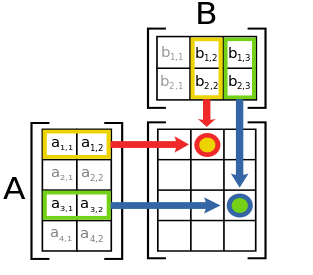
\includegraphics{images/matrix_mult.png}
\caption{matrix mult}
\end{figure}

Looking at it this way, left-rows and right-columns triangulate the
output values of the product. For brevity, we won't present a full
formula here, and like usual we can just use the \texttt{.dot()} numpy
method from one array onto another to execute this computationally:

    \begin{Verbatim}[commandchars=\\\{\}]
{\color{incolor}In [{\color{incolor}58}]:} \PY{c+c1}{\PYZsh{}\PYZsh{} define a 4\PYZhy{}row by 3\PYZhy{}column matrix}
         \PY{n}{A} \PY{o}{=} \PY{n}{np}\PY{o}{.}\PY{n}{array}\PY{p}{(}\PY{p}{[}
             \PY{p}{[} \PY{l+m+mi}{1}\PY{p}{,}  \PY{l+m+mi}{2}\PY{p}{,}  \PY{l+m+mi}{3}\PY{p}{]}\PY{p}{,}
             \PY{p}{[} \PY{l+m+mi}{4}\PY{p}{,}  \PY{l+m+mi}{5}\PY{p}{,}  \PY{l+m+mi}{6}\PY{p}{]}\PY{p}{,}
             \PY{p}{[} \PY{l+m+mi}{7}\PY{p}{,}  \PY{l+m+mi}{8}\PY{p}{,}  \PY{l+m+mi}{9}\PY{p}{]}\PY{p}{,}
             \PY{p}{[}\PY{l+m+mi}{10}\PY{p}{,} \PY{l+m+mi}{11}\PY{p}{,} \PY{l+m+mi}{12}\PY{p}{]}
         \PY{p}{]}\PY{p}{)}
         
         \PY{n+nb}{print}\PY{p}{(}\PY{n}{A}\PY{p}{,} \PY{l+s+s1}{\PYZsq{}}\PY{l+s+se}{\PYZbs{}n}\PY{l+s+s1}{\PYZsq{}}\PY{p}{)}
         
         \PY{c+c1}{\PYZsh{}\PYZsh{} define a 3\PYZhy{}row by 2\PYZhy{}column matrix}
         \PY{n}{B} \PY{o}{=} \PY{n}{np}\PY{o}{.}\PY{n}{array}\PY{p}{(}\PY{p}{[}
             \PY{p}{[} \PY{l+m+mi}{11}\PY{p}{,}  \PY{l+m+mi}{12}\PY{p}{]}\PY{p}{,}
             \PY{p}{[} \PY{l+m+mi}{13}\PY{p}{,}  \PY{l+m+mi}{14}\PY{p}{]}\PY{p}{,}
             \PY{p}{[} \PY{l+m+mi}{15}\PY{p}{,}  \PY{l+m+mi}{16}\PY{p}{]}\PY{p}{,}
         \PY{p}{]}\PY{p}{)}
         
         \PY{n+nb}{print}\PY{p}{(}\PY{n}{B}\PY{p}{,} \PY{l+s+s1}{\PYZsq{}}\PY{l+s+se}{\PYZbs{}n}\PY{l+s+s1}{\PYZsq{}}\PY{p}{)}
         
         \PY{c+c1}{\PYZsh{}\PYZsh{} take the inner matrix product}
         \PY{c+c1}{\PYZsh{}\PYZsh{} which results in a 4 x 2 matrix}
         \PY{n+nb}{print}\PY{p}{(}\PY{n}{A}\PY{o}{.}\PY{n}{dot}\PY{p}{(}\PY{n}{B}\PY{p}{)}\PY{p}{)}
\end{Verbatim}


    \begin{Verbatim}[commandchars=\\\{\}]
[[ 1  2  3]
 [ 4  5  6]
 [ 7  8  9]
 [10 11 12]] 

[[11 12]
 [13 14]
 [15 16]] 

[[ 82  88]
 [199 214]
 [316 340]
 [433 466]]

    \end{Verbatim}

    \hypertarget{eigenvectors-and-eigenvalues}{%
\paragraph{1.1.4.8 Eigenvectors and
Eigenvalues}\label{eigenvectors-and-eigenvalues}}

While there's a lot of depth in this discussion that we'll have to
avoid, the topic of eigenvectors is essential when thinking of linear
algebra and matrices as modeling tools. The important concept with
eigenvectors that we want to discuss has to do with matrix-times vector
multiplication. Recall: an \((m \times n)\) matrix \(A\) times an
\((n \times 1)\) vector \(v\) results in another vector, having
dimension \((m \times 1)\). So what if \(m = n\), i.e., the matrix \(A\)
is \emph{square}? Well, then we could take the result and multiply it by
\(A\) again! This is one of the things that eigenvectors are all about:

\begin{itemize}
\tightlist
\item
  if \(A\) is an \((n \times n)\) matrix and \(v\) is an eigenvector of
  \(A\), then for some non-zero scalar (constant), \(\lambda\):
\end{itemize}

\[A\cdot v = \lambda v\]

\(\lambda\) is called the eigenvector's \emph{eigenvalue}. In other
words, matrix-times-eigenvector returns a vector that points in the same
exact direction as the original eigenvector. You can keep multiplying
the result by \(A\) and get back scalings, i.e., growing/shrinking of
the same vector. Later on, when we get into our discussion of networks
we'll get to see how Google used this eigenvector concept this to build
their PageRank algorithm, which truly enabled them to take over the web
search market.

So, how do you find these magical eigenvectors? That's a bit more of a
tricky problem, and as it turns out a matrix has \(n\) eigenvectors
(they may just not all be real). However, since we're not going to be
worrying about doing linear algebra by hand, we won't get into it here.
Instead, let's just look at what comes for free with numpy via
\texttt{numpy.linalg.eig()}:

    \begin{Verbatim}[commandchars=\\\{\}]
{\color{incolor}In [{\color{incolor}59}]:} \PY{c+c1}{\PYZsh{}\PYZsh{} define a 2\PYZhy{}row by 2\PYZhy{}column matrix}
         \PY{n}{A} \PY{o}{=} \PY{n}{np}\PY{o}{.}\PY{n}{array}\PY{p}{(}\PY{p}{[}
             \PY{p}{[} \PY{l+m+mi}{1}\PY{p}{,}  \PY{l+m+mi}{2}\PY{p}{]}\PY{p}{,}
             \PY{p}{[} \PY{l+m+mi}{4}\PY{p}{,}  \PY{l+m+mi}{5}\PY{p}{]}
         \PY{p}{]}\PY{p}{)}
         
         \PY{n+nb}{print}\PY{p}{(}\PY{n}{A}\PY{p}{,} \PY{l+s+s1}{\PYZsq{}}\PY{l+s+se}{\PYZbs{}n}\PY{l+s+s1}{\PYZsq{}}\PY{p}{)}
         
         \PY{n}{e\PYZus{}vals}\PY{p}{,} \PY{n}{e\PYZus{}vecs} \PY{o}{=} \PY{n}{np}\PY{o}{.}\PY{n}{linalg}\PY{o}{.}\PY{n}{eig}\PY{p}{(}\PY{n}{A}\PY{p}{)}
         
         \PY{c+c1}{\PYZsh{}\PYZsh{} the list of eigenvalues}
         \PY{n+nb}{print}\PY{p}{(}\PY{n}{e\PYZus{}vals}\PY{p}{,} \PY{l+s+s1}{\PYZsq{}}\PY{l+s+se}{\PYZbs{}n}\PY{l+s+s1}{\PYZsq{}}\PY{p}{)}
         
         \PY{c+c1}{\PYZsh{}\PYZsh{} the columns are our eigenvectors}
         \PY{n+nb}{print}\PY{p}{(}\PY{n}{e\PYZus{}vecs}\PY{p}{,} \PY{l+s+s1}{\PYZsq{}}\PY{l+s+se}{\PYZbs{}n}\PY{l+s+s1}{\PYZsq{}}\PY{p}{)}
         
         \PY{c+c1}{\PYZsh{}\PYZsh{} multiplying A by a column and dividing by }
         \PY{c+c1}{\PYZsh{}\PYZsh{} its eigenvalue results in the exact same column/eigenvector}
         \PY{n+nb}{print}\PY{p}{(}\PY{n}{A}\PY{o}{.}\PY{n}{dot}\PY{p}{(}\PY{n}{e\PYZus{}vecs}\PY{p}{[}\PY{p}{:}\PY{p}{,} \PY{l+m+mi}{0}\PY{p}{]}\PY{p}{)} \PY{o}{/} \PY{n}{e\PYZus{}vals}\PY{p}{[}\PY{l+m+mi}{0}\PY{p}{]}\PY{p}{)}
\end{Verbatim}


    \begin{Verbatim}[commandchars=\\\{\}]
[[1 2]
 [4 5]] 

[-0.46410162  6.46410162] 

[[-0.80689822 -0.34372377]
 [ 0.59069049 -0.9390708 ]] 

[-0.80689822  0.59069049]

    \end{Verbatim}

    \hypertarget{but-what-do-eigenvectors-and-eigenvalues-mean-intuitively}{%
\paragraph{1.1.4.9 But what do eigenvectors and eigenvalues mean,
intuitively?}\label{but-what-do-eigenvectors-and-eigenvalues-mean-intuitively}}

Geometrically, eigenvectors tell you the directions along which your
data spread out. This means we can use eigenvectors to tell us about the
variation present in a spreadsheet of data, i.e., about how columns and
rows of data covary. So, if each point in a data set is a row,
represented by two variable columns, we would be able to use
eigenvectors to show us something like:

\begin{figure}
\centering
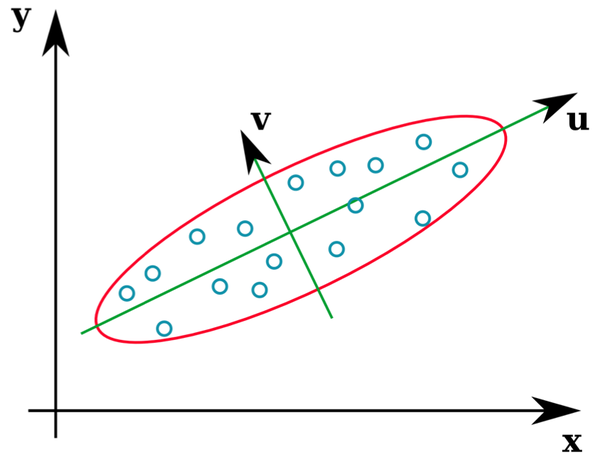
\includegraphics{images/eigenvectors.png}
\caption{eigen}
\end{figure}


    % Add a bibliography block to the postdoc
    
    
    
    \end{document}
